\documentclass[12pt]{ucthesis}

\usepackage{etex}
\usepackage[morefloats=125]{morefloats}
\usepackage[hyphens]{url}
% \usepackage{subfig}
\usepackage{graphicx}
\usepackage{tabularx}
\usepackage{amssymb}
\usepackage{amsmath}
\usepackage{bm}
\usepackage[letterpaper]{geometry}
\usepackage[overload]{textcase}
\usepackage{color}
\usepackage[nonumberlist,toc]{glossaries}
\usepackage{wrapfig}
\usepackage{longtable}
\usepackage{morefloats}
\usepackage{float}
\usepackage{listings}
\usepackage{makecell}
\usepackage{appendix}
% \usepackage[]{algorithm2e}
\usepackage{algorithm,algpseudocode} % https://tex.stackexchange.com/a/230789
\usepackage{titlesec}
\usepackage[breaklinks=true,hidelinks,pdfusetitle]{hyperref}
\usepackage{cleveref}
\usepackage{ifthen}
\usepackage{lmodern,microtype,enumitem,todonotes,booktabs,multirow,subcaption}
% \usepackage{minted}
\usepackage[export]{adjustbox}
\usepackage{pgfplots}

\lstdefinestyle{default}{
  basicstyle=\footnotesize\ttfamily,
  breaklines=true,
  language=C,
  captionpos=b,
  numbers=left,
  frame=single
}
\lstset{style=default}
\renewcommand*{\lstlistlistingname}{LIST OF LISTINGS}

\graphicspath{ {figures/} }

\makeindex
\makeglossaries

% Shrink the size of headers
\titleformat{\chapter}[display]
        {\normalfont\normalsize\centering}
        {\ifthenelse{\equal{\thechapter}{A}}{APPENDICES\\[4.3ex]}{}\chaptertitlename\ \thechapter}
        {0pt}{\normalsize\uppercase}
\titlespacing*{\chapter}{0pt}{-20pt}{4.3ex plus .2ex}


\titleformat*{\section}{\normalsize\bfseries}
\titleformat*{\subsection}{\small\bfseries}
\titleformat*{\subsubsection}{\small\bfseries}
\titleformat*{\paragraph}{\small\bfseries}
\titleformat*{\subparagraph}{\small\bfseries}

\bibliographystyle{abbrv}

\setlength{\parindent}{0.25in} \setlength{\parskip}{6pt}
\geometry{verbose,nohead,tmargin=1in,bmargin=1in,lmargin=1.5in,rmargin=1in}
\setcounter{tocdepth}{2}

% Different font in captions (single-spaced, bold) ------------
\newcommand{\captionfonts}{\small\bf\ssp}

\newcommand{\mycaption}[2]{\caption[#1 --- #2]{#1 --- #2}}

\makeatletter  % Allow the use of @ in command names
\long\def\@makecaption#1#2{%
  \vskip\abovecaptionskip
  \sbox\@tempboxa{{\captionfonts #1: #2}}%
  \ifdim \wd\@tempboxa >\hsize
    {\captionfonts #1: #2\par}
  \else
    \hbox to\hsize{\hfil\box\@tempboxa\hfil}%
  \fi
  \vskip\belowcaptionskip}
\makeatother   % Cancel the effect of \makeatletter
% ---------------------------------------

% Define Appendix refs
\crefname{app}{appendix}{appendices}
\Crefname{app}{Appendix}{Appendices}

\begin{document}

% Declarations for Front Matter
\title{Your Thesis Title}
\author{Your Name}
\degreemonth{June} \degreeyear{2014} \degree{Master of Science}
\defensemonth{June} \defenseyear{2014}
\numberofmembers{2}
   \chair{Alexander Dekhtyar, Ph.D. \linebreak Professor of Computer Science}
   \othermemberA{Aaron Keen, Ph.D. \linebreak Professor of Computer Science}
   \othermemberB{Franz Kurfess, Ph.D. \linebreak Professor of Computer Science}
\field{Computer Science} \campus{San Luis Obispo}
\copyrightyears{seven}


\maketitle

\begin{frontmatter}

% Custom made for Cal Poly (by Mark Barry, modified by Andrew Tsui).
\copyrightpage

% Custom made for Cal Poly (by Andrew Tsui).
\committeemembershippage

\begin{abstract}
Modeling believable lighting is a crucial component of computer graphics applications, including games and modeling programs. Physically accurate lighting is complex and is not currently feasible to compute in real-time situations. Therefore, much research is focused on investigating efficient ways to approximate light behavior within these real-time constraints.

In this thesis, we implement a general purpose algorithm for real-time applications to approximate indirect lighting. Based on voxel cone tracing~\cite{crassin2011interactive}, we use a filtered representation of a scene to efficiently sample ambient light at each point in the scene. We present a novel approach to scene voxelization using hardware tesselation and compare it with an approach utilizing hardware rasterization. We also investigate possible methods of nonuniform voxelization.

Our contributions include a complete and open-source implementation of voxel cone tracing along with both voxelization algorithms. We find similar performance to the raster approach approach but with promising results for perspective warped voxels.

%We also extend the base algorithm to better accomodate large scenes by applying a warping function to our filtered representation. This allows us to increase lighting detail near the camera without a significant increase in memory usage or a performance penalty.

%Final results show real-time performance and good lighting quality largely independent of screen and scene size. In addition, the implementation is open-source, cross-platform, and easy to integrate into existing engines.
\end{abstract}

\begin{acknowledgements}
\noindent
Thanks to:
\begin{itemize}
    \item My parents, for always supporting me
    \item My brother, Jake, for being a bro
    \item My friends, for the encouragement, laughs, and fun
    \item The wonderful professors at Cal Poly, most notably Dr.~Zo\"e Wood and Dr.~Christian Eckhardt
    \item Andrew Guenther, for uploading this template
\end{itemize}

\end{acknowledgements}

\tableofcontents

\listoftables

\listoffigures

% \lstlistoflistings
% \addcontentsline{toc}{chapter}{LIST OF LISTINGS}
% \addtocontents{lol}{Listing \hfill Page}

% Add CHAPTER into table of contents.
\addtocontents{toc}{%
   \noindent CHAPTER
}

\end{frontmatter}

\pagestyle{plain}

\renewcommand{\baselinestretch}{1.66}

\chapter{Introduction}
Computer graphics is the task of taking a virtual description of a scene, composed of objects such as models and lights, and rendering that scene to an image. One of the core components involved with this is computing realistic lighting. Although light behavior is fairly well understood in the physical sense, accurately simulating this behavior is a heavy computational task. The goal in computer graphics, then, is how to efficiently approximate light behavior where there are time and resources constraints.

% TODO paragraph or subsection about raytracing/offline gi somewhere?

Of particular importance in computer graphics are real-time applications, where images, or frames, must be produced at an interactive speed, such as video games. Typically, the lower bound for this is considered 30 frames per second, or about 33 milliseconds per frame, and a target of 60 frames per second, or about 17 milliseconds per frame. To meet this goal, researchers and engineers have designed many algorithms and techniques.
% TODO reword
In this work, we implement and extend an algorithm to accomplish fast and accurate lighting for fully dynamic scenes. An example of our global illumination algorithm is shown in Figure~\ref{fig:introduction_gi}.

% TODO seems like a good thing to note (it's very engineer-y)
It is important to keep in mind that most lighting algorithms have many tradeoffs and are adapted towards specific use cases. A complete lighting system may also combine many different lighting algorithms in order to achieve the desired balance between quality, performance, and ease of use.

\begin{figure}[h]
\centering
    \begin{subfigure}[t]{0.4\textwidth}
        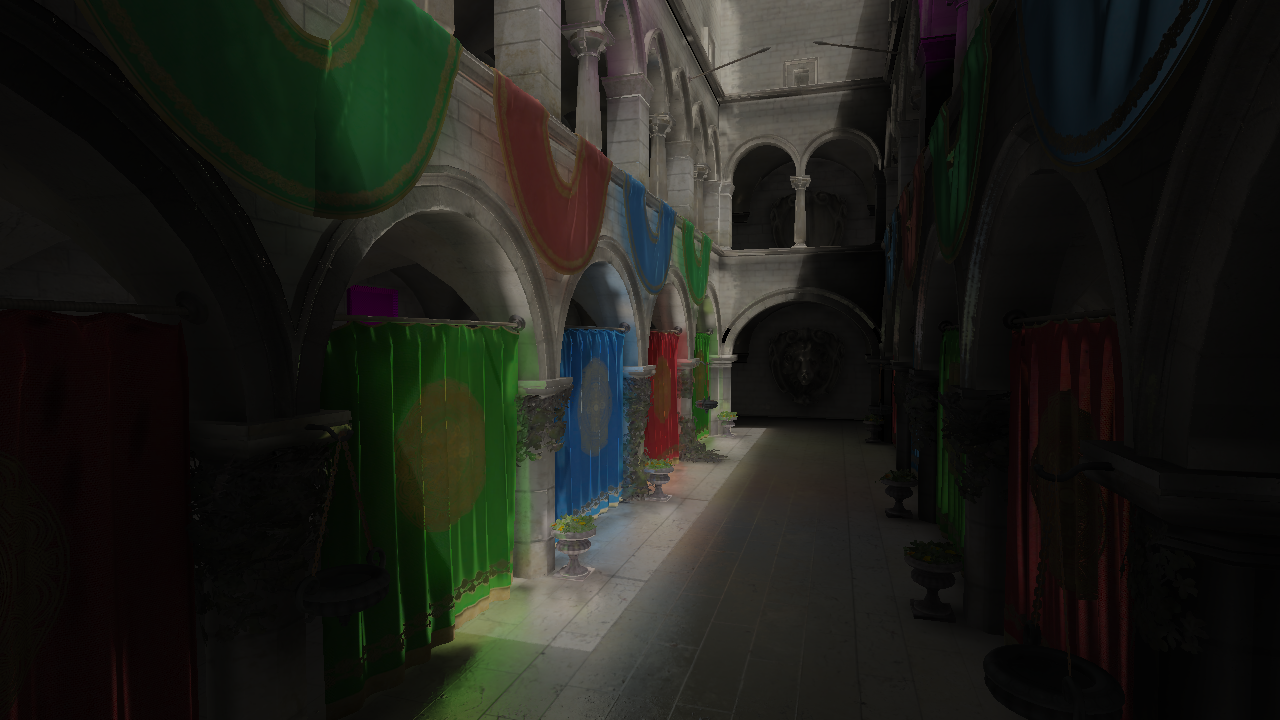
\includegraphics[width=\textwidth]{gi_on.png}
        \caption{Global illumination}
    \end{subfigure}
    ~
    \begin{subfigure}[t]{0.4\textwidth}
        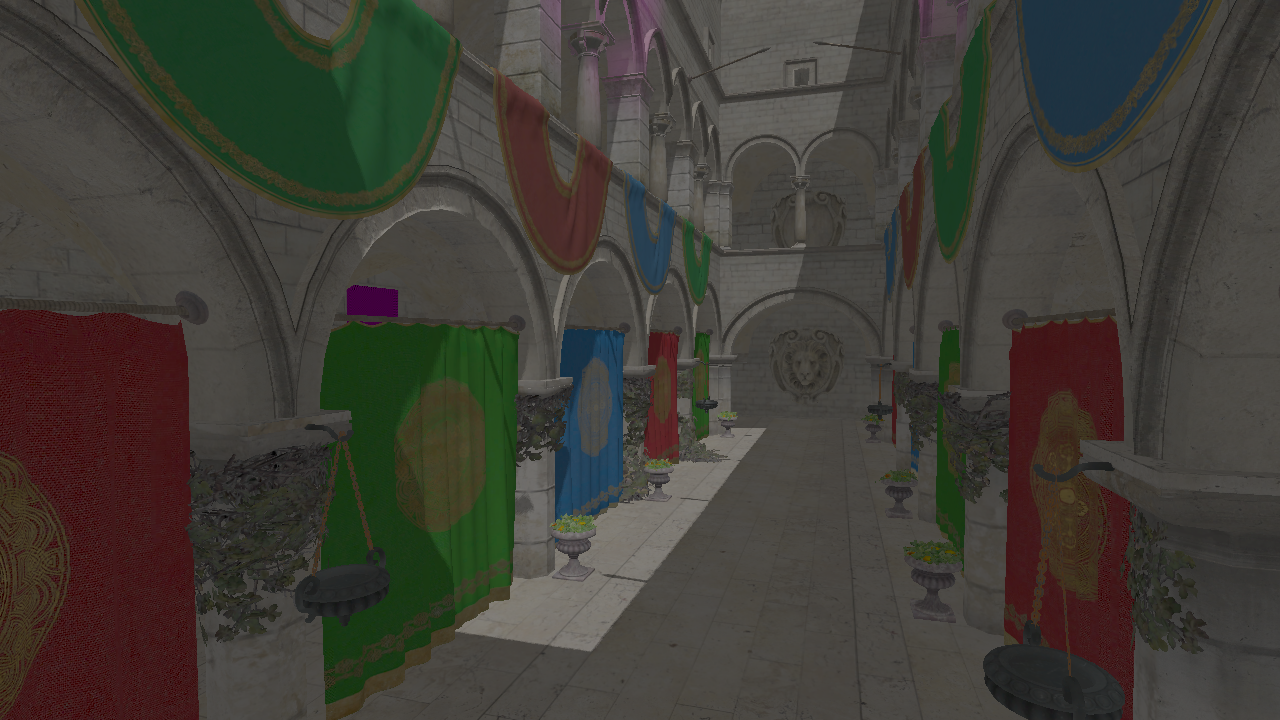
\includegraphics[width=\textwidth]{gi_off.png}
        \caption{No global illumination}
    \end{subfigure}
    \caption{A scene---describing information like light sources, materials, and geometry---is rendered by computing a color for each pixel of a screen. The image on the left is rendered with global illumination whereas the image on the right uses a constant ambient term for indirect lighting.}
    \label{fig:introduction_gi}
\end{figure}

\section{Real-Time Global Illumination}
In general, lighting at a given point is a combination of direct and indrect light. Direct light is light accumulated directly from a light source, whereas indirect light is the light that comes from other non-light sources in the scene (e.g.\ the light that has `bounced' off of objects in the scene).

% TODO ambient occlusion: footnote with citations for a few types (SSAO, HBAO, etc.)
% TODO cite specific sections of book howdo?
In the beginnings of computer graphics simple lighting models were used in order to maintain real-time performance. While the direct light was feasible to compute in real-time (albeit with limitations on number of lights and other optimizations), indirect lighting was often faked with a simple constant contribution. As hardware limitations and algorithms improved, more advanced techniques were developed and approximating the indirect light became more feasible. Two methods, ambient occlusion~\cite{bunnell2005dynamic,moller2008rtr} and baked lighting~\cite{Sloan:2002:PRT:566654.566612,moller2008rtr}, became standard ways of introducing simple global illumination, the term given to techniques that improved indirect lighting. However both these methods have drawbacks. Ambient occlusion, which approximates the effect of light occlusion by nearby objects, provides a great improvement over the constant ambient term used previously but does not accurately simulate the indirect light in its entirety. Thus it is only `partial' global illumination. Baked lighting involves pre-computing light behavior of a scene prior to runtime and then utilizing the precomputation to enable real-time realistic lighting. The drawback here is only static objects can have their light baked---any dynamic objects or lights in the scene are not accounted for.

% TODO reword
Full global illumination algorithms attempt to provide a complete approximation of indirect light. Some, like baked lighting, only work for static scenes. For our work, however, we are interested in dynamic global illumination. In other words, our goal is full global illumination that can be performed completely for each frame. Any changes in the scene---object movement, light movement or changes in intensity---will be accounted for.

For dynamic real-time global illumination, a common approach is to first construct a spatial representation of a scene's radiance (light information) and then use that representation to approximate the radiance at a given point in the scene. Popular methods that follow this approach are light propagation volumes~\cite{Kaplanyan:2010:CLP:1730804.1730821} and voxel cone tracing~\cite{crassin2011interactive} (see Related Works for more). Some challenges that arise from methods like these are issues with GPU memory consumption and achieving adequate lighting detail. % TODO expand on these problems more?

\section{Our Contribution}
% TODO should I put results here too?
The main contribution of this work is a complete implentation of computing global illumination based on voxel cone tracing with a focus on ease of use and speed while still producing high quality results. We hope this provides a competitive alternative to existing real-time global illumination systems that can be used for educational purposes.

 We also present an approach to scene voxelization using hardware tessellation and compare it with an approach utilizing hardware rasterization. We find similar performance to the raster approach approach but with promising results for perspective warped voxels. We also investigate possible methods of nonuniform voxelization.

%The novel contribution, voxel warping, is a way to handle large scenes in a memory efficient and simple way. The idea is to adjust the voxel density of the scene based on its distance from the camera, which allows a large scene to be represented without requiring large memory or performance overheads.

% TODO fact check and citations needed
Another important part of our contribution is that the implementation is open-source (under the MIT license) and cross platform (on Linux and Windows using modern OpenGL\footnote{macOS is not supported since Apple only supports up to OpenGL 4.1~\cite{appleopenglsupport}, whereas we require 4.5 (for features like compute shaders, direct state access, and image objects).}. Many graphics implementations are developed in the research or industrial space and are often not made available to the public for various reasons (e.g.\ copyright). Even implementations that are openly available often are tied to a specific game engine or other large codebase\footnote{For example, NVIDIA's VXGI is integrated into a custom branch of Unreal Engine 4 (distributed as a binary)~\cite{nvidiavxgi} and Light Propogation Volumes are implemented in CryEngine3~\cite{kaplanyan2009light}. The Godot engine~\cite{godotengine} is a notable exception here and, while part of a large codebase, is relatively small and is completely open source.}, making it difficult to understand or integrate into one's own project. Furthermore, many implementations utilize DirectX as their graphics API, which limits the implementation to Windows only. We hope that providing an easy to understand and cross platform implementation will help others learn more about voxel cone tracing and dynamic real-time global illumination.

\chapter{Background}

\section{Voxelization}
To develop an interactive 3D application, some kind of representation for the scene is needed. Traditionally, all geometric objects in a scene are represented by triangles. For example, to model a simple cube we can represent each of its faces using two triangles for a total of 12 triangles. The reason for using triangles is due to their geometric simplicity (triangles contain the fewest number of points that define a plane). Also, as dedicated Graphics Processing Units (GPUs) became more common they were designed with this traditional triangle rasterization in mind so they have specialized hardware to operate on triangles. In other words, triangles are fast to process.

But triangles do have some issues. Primarily, they do a good job of referencing surfaces (since they are inherently 2D) but they don't lend themselves well to volumetric (3D) data. For example, a natural representation of a cloud would be a 3D volume representing the density of the cloud at a given point within the volume. There are algorithms that can convert from a volumetric representation to a triangle one---marching cubes being the most popular---but it still only models an arbitrary isosurface as opposed to the actual volume.

Voxels (volume elements) represent 3D objects in a natural way. A volumetric representation of an object is a 3D grid of cells (the voxels) which hold any data relevant to that voxel: color, transparency, and normal, to name a few. Recently, voxels have grown popular in the computer graphics field due to this natural representation of 3D objects. The main reason voxels were not used much in the past is mainly due to the amount of memory required to store a voxelized representation as well as GPUs being specialized for triangle rasterization (and not being easy for more general purpose computing). This restriction has largely been lifted since modern GPUs have much more memory and general purpose GPU (GPGPU) computing has allowed programmers to work more easily with non-triangle based computing.

\section{Radiance and the Rendering Equation}
In order to render a scene, we need some model of how light works.
<explain radiance>
<show rendering equation>
Of course, in order to do this on a computer we must at the very least discretize the problem. Furthermore, the complexity involved in calculating all of the integrals that would be needed as stated by the rendering equation is computationally infeasible. Thus we need some way to approximate this complete model of light.

\section{Global Illumination}
The term global illumination generally refers to a lighting model which attempts to accurately approximate indirect illumination. Approaches like having a constant ambient light amount and using ambient occlusion techniques like SSAO and HBAO do try to emulate some of the effects of global illumination but do not really attempt to accomplish full global illumination. Here we give an overview of some techniques used to achieve global illumination.

\subsection{Raytracing}

\subsection{Baked Lighting}

\subsection{Full Dynamic Global Illumination}





Representing Geometry
    Triangle Rasterization
    Voxels - like a pixel but 3d

Radiance and the Rendering Equation
    combo of direct + indirect, expensive to do perfectly

Global Illumination
    need ways of approximating. some simple hacks are constant diffuse term, AO
    more advanced methods needed...

    Raytracing (Monte Carlo)
        transition with but not real time... (even with things like photon mapping)
    Baked Lighting
        but this doesnt handle dynamic lighting...
    Full GI
        Voxel Cone Tracing
        VPLs, light probes?
        The other NVIDIA one?

\chapter{Related Work}

Global illumination is a broad term that can be approached in many ways. With respect to this thesis, we only focus on comparisons with other real-time, fully dynamic techniques. Many of these techniques borrow similar ideas and build off of each other. The implementations for a single technique can also vary greatly based on data structures used, shading models, and other considerations. The different tradeoffs made and how they affect the final implementation are important to understand, as there is often not a single best way to approach the problem of global illumination. Here we present some of the more popular and relevant methods of achieving full global illumination and attempt to note the major differences between them and our implementation.

\section{Reflective Shadow Maps}
Dachsbacher and Stamminger introduced RSMs in 2005. Their work extends off of traditional shadow mapping to support single bounce indirect illumination. The main idea is to treat each pixel in the shadow map---each pixel in the shadow map corresponds to a directly lit point---as a virtual point light (VPL) which illuminates the rest of the scene~\footnote{VPLs were introduced in the paper TODO}. In order to efficiently compute the contribution of the VPLs for a point in the scene a fixed number of samples are taken from the shadow map. They also apply an interpolation scheme to reduce computation on smooth parts of the scene.

A notable downside of this method is occlusion information is not accounted for: a point $y$ could contribute indirect lighting to another point $x$ even if there is other geometry blocking the path between $x$ and $y$. The authors apply a separate ambient occlusion pass to partially mitigate this problem. The method is also only designed for low frequency lighting details. Also, while directional, point, and spot lights should theoretically work, objects that themselves emit light were not addressed.

\section{Light Propogation Volumes}
LPVs are another method for approximating low frequency indirect lighting, create by Kaplanyan and Dachsbacher in 2010. The method relies on an iterative based light propogation algorithm within a volumetric grid structure. This structure, the LPV, is initialized by injecting VPLs into its cells---for example, by using RSMs. Next, the light is propogated multiple times between adjacent cells; each propogation results in the LPV having a more complete representation of the indirect light in the scene.

LPVs improve on (TODO RSM PAPER) by essentially filtering the light in multiple steps. It also stores low resolution geometry information for occlusion purposes. They also tackle the issue of handling large scenes with the concept of cascaded LPVs: multiple individual LPV structures are used with different sizes, focusing detail near the camera. Essentially, the LPV is a clipmap.
% TODO do I nee dto list everything they did?

% TODO do authors mention performance or memory cost of adding their improvements?
The main drawback of this method is the lighting is low frequency only. Proper glossy (specular) reflections are still wanted in many applications. Also, the geometry information obtained is not complete: it is created by reusing other results from shadow mapping and depth peeling.

\section{GPU Pro 4}
Rasterized Voxel-Based Dynamic Global Illumination described by Doghramachi in ???? is based heavily on LPVs but uses a voxelized scene representation for the initial steps of LPV creation. This avoids some of the difficulties when injecting VPLs as in the LPV paper. In addition, the geometry information made available by voxelization is complete and does not require external inputs like shadow maps or depth peeling.

Just like LPVs, the main downside here is lack of specular reflections, which stems from the low resolution grid used for the LPV (32x32x32, as mentioned in the implementation, whereas we aim for somewhere on the order of $128^3$ to $256^3$). Also, the method does suffer from some light leaking due to how point lights are injected into the scene: instead of creating an RSM (which handles occlusion properly), all voxels within a defined distance of the point light are injected into the initial LPV.

\section{Voxel Cone Tracing}
In 2011, Crassin et al.\ introduced Interactive Indirect Illumination Using Voxel Cone Tracing. A primary improvement over the existing methods sought in this method was to obtain higher frequency lighting details, such as specular reflections. The core idea to balance performance  with lighting detail is to make use of a filtered radiance representation which is then sampled using voxel cone tracing, a concept they introduce.

The first step in the algorithm is to create a high resolution radiance representation. Crassin et al.\ inject radiance into the leaves of an octree using the familiar RSM technique. An octree is used to reduce memory consumption, a consequence of using such a high resolution radiance representation. The octree is then filtered recursively bottom up until all inner nodes in the octree have a filtered radiance value. The final step, voxel cone tracing, is essentially a combination of raymarching and mipmapping: samples come from successively lower levels of detail.

% TODO move the section on vct from implementation here instead?
% TODO by varying the angle of the cone, different affects can be replicated: large -> diffuse, small -> specular

Although the octree representation does help alleviate issues when dealing with sparse scenes, GPU memory consumption is still an issue especially for larger scenes. In addition, due to their tree-like nature, octrees are awkward for GPU use and do not benefit from things like hardware supported texture filtering. To address this, NVIDIA decided to use a clipmap instead of an octree in their standard implementation of voxel cone tracing, VXGI.

% TODO explain why warping may be better approach: simpler (one texture), memory use, easily configurable, better suited to large scenes?

\iffalse
% TODO forward+ indirect?

* Global Illumination using Voxel Cone Tracing
- octrees vs clipmaps vs 3d textures (vs warped)
- proprietary
- vxgi: clipmaps, in UE4 but still closed source
    - octree -> no hw filtering, complex but higher resolution
    - multiple levels of radiance -> allows gathering more high frequency indirect lighting information

* some common issues with other works (this could also go in intro)
- closed source
- implementation details matter -> difficult to understand from research or white papers
- highly variable performance based on unrelated things (OpenGL vs DirectX? modern OpenGL? mipmaps, normal maps, shading model, mesh optimizations, etc)
- research renderers or full game engines -> difficult to understand
\fi
\chapter{Validation}

\section{Expected Results}
The primary deliverable of this work is a real-time global illumination algorithm. Naturally, the two primary measures of success for this will be the execution time and the visual quality. Execution time is simple to evaluate: the execution time required for the algorithm as well as the frame time for the entire program can be timed. This will provide a good way of comparing this global illumination method to others. It also provides a way to measure how the algorithm scales with various parameters such as screen resolution and geometric complexity. Visual quality is difficult to objectively define, so simple comparisons to other methods is preferable. There are a few visual qualities that are a requirement for the algorithm: ambient occlusion, color bleeding, specular reflections, and little to no light leaking. These specific qualities can be used as a rough indicator of how well the global illumination algorithm performs.

\section{Methodology}
The first part of the validation plan will be to create multiple test scenes that will showcase the desired properties of the algorithm. The test scenes chosen will be

\begin{enumerate}
\item[Sponza: ] This scene is a de facto standard environment of moderate geometric complexity. There are multiple areas that showcase interesting lighting as well as specular reflections, color bleeding, and light leaking.
\item[San Miguel: ] Another popular scene used to showcase new lighting algorithms.
\item[Light Leak Test: ] This custom test scene is designed to exhibit light leaking and will be a good indicator of how well our algorithm addresses that issue.
\end{enumerate}

Comparisons between no global illumination, our algorithm, and NVIDIA's VXGI will be shown and analyzed for the given scenes.

In terms of evaluating the algorithm by itself, we can examine how changing screen resolution, geometric complexity, number of lights, and voxelization dimension will affect the algorithm. 


\chapter{Methodology}

???
1. Implement basic voxel cone tracing (with 3d texture)
2. Investigate how to extend to larger scene without significant increase in memory, computation, or complexity
3. Figuring out warp function and comparing it with linear version?
\chapter{Implementation}

At its core, the application we created for this thesis is a standard forward rendering engine supporting multiple lights, shadow mapping, and normal mapping---in addition, of course, to full real-time dynamic global illumination. The scene to be rendered is composed of one or more actors, which are simply meshes loaded from the generic Wavefront OBJ file format. Actors are also capable of rigid body animations.

The rendering pipeline can be broken down into several render passes, each of which will be explained in its corresponding section. In general, the main steps taken are generating a voxelized representation of the scene, creating a filtered representation of light from the voxels and light sources, and, finally, shading the scene.

The application itself is written in C++11 and uses OpenGL as the graphics API. In order to make use of modern graphics features like compute shaders and direct state access we require OpenGL version 4.5 (released in 2014). The project uses CMake as its build system and has been tested on Linux and Windows.

% TODO should I mention conventions used for variables and such?

% TODO using tinyobj w/ http://exocortex.com/blog/extending_wavefront_mtl_to_support_pbr for pbr
% PBR shading (Cook-Torrance, Disney, UE4, ...) https://disney-animation.s3.amazonaws.com/library/s2012_pbs_disney_brdf_notes_v2.pdf

% TODO include code snippets, API calls, diagrams
%TODO name the 3D texture (and refer to it in monospace)?
\section{Voxelization} \label{sec:voxelization}
The goal of voxelization is to create a sparse 3D representation of the geometry in the scene. The information associated with each voxel is stored in two 3D textures: one for color and opacity and another for surface normal. We refer to these textures as \texttt{voxelColor} and \texttt{voxelNormal}, respectively. Each texture has an internal format of \texttt{RGBA16F} or \texttt{RGBA8}, depending on hardware capabilities. The resolution of the textures is configurable at runtime, although the default is $256^3$.

The extents of our voxelization volume---the area in world space that will end up inside the voxel textures---is also configurable and by default is set to enclose the entire scene. This volume can be static or can track the camera (with the camera being at the center of the textures). In addition, to prevent some issues with temporal artifacts, the voxel textures are snapped to a discrete grid corresponding to the size of each voxel cell in world space.

We present two different approaches for scene voxelization: one utilizing hardware rasterization and the other hardware tessellation.

\subsection{Rasterization-Based Approach to Voxelization}
% TODO scene extents, midpoint and tracking, computing voxel texture coordinates, choosing axis, diagram of scene extents and converting to NDC
% TODO cite GPU Pro 4 and imageAtomicMax
The first method for voxelization utilizes the GPU rasterization pipeline and is based on~\cite{crassin2012octree}. The voxelization is performed completely in a single render pass. The basic idea is to rasterize the scene such that each fragment generated by the GPU corresponds to a single voxel in the 3D texture.

One of the main challenges with voxelization is ensuring there are no holes or cracks in the resulting grid. Two techniques are used to mitigate this (and will be covered in-depth in the following paragraphs). First, for each triangle we project along the triangle's normal's dominant axis. This maximizes the number of fragments generated for a given triangle. Second, we perform conservative rasterization. Normally, the GPU only generates a fragment for a given pixel if a triangle overlaps the center of the corresponding pixel. This results in cracks in the voxelized grid since even if a triangle is inside a voxel it may not be rasterized.

Before the draw call, the necessary matrices to project the geometry into the voxelization volume are created. The projection matrix is orthographic, with bounds corresponding to the extents of the voxelization volume. In order to project along each triangle's dominant axis, we also need three view matrices: for each axis a view matrix is constructed where the view position is at the edge of the voxel volume and looks down its respective axis. The final matrix used to transform a point in world space to a point in the voxel texture for a particular axis is composed by multiplying the orthographic matrix with the appropriate view matrix.

% TODO what do with this
For the shader program, the voxel textures are bound as \texttt{image3D} objects (as textures are read-only in shaders). Following from that, since the framebuffer is not being written to, color writing is disabled. Lastly, depth testing and depth writes are also disabled, since the goal is to voxelize the entire scene. The algorithm is shown in Algorithm~\ref{alg:voxelization} and explained in detail below.

\begin{algorithm}
    \caption{Voxelization}
    \label{alg:voxelization}
    \begin{algorithmic}
        \For {each triangle $t$}
        \State {find dominant axis of $t$ using surface normal}
        \State {apply projection matrix corresponding to the dominant axis}
        \EndFor
        \State{Rasterization}\Comment {Performed by hardware}
        \For {each rasterized fragment} \Comment {position is in NDC}
        \State {transform NDC coordinates to texture space ($[0, 1]$)}
        \State {Realign NDC coordinates with standard coordinate system}
        \State {Insert fragment into voxel texture}
        \EndFor
    \end{algorithmic}
\end{algorithm}

Starting in the vertex shader, the only operation performed is transforming the object from object space to world space using its appropriate model matrix. In the geometry shader we take a single triangle in world space, transform it based on its dominant axis, and output the resulting triangle in clip space. The triangle's dominant axis is determined by finding the largest component of its normal (by absolute value)\footnote{Finding the dominant axis is really finding the maximum dot product of each axis with the normal, but since we use the standard basis this reduces to just finding the largest component of the normal.}. We then apply the appropriate projection matrix according to the dominant axis and output the resulting triangle to be rasterized. In the fragment shader, each fragment's position in Normalized Device Coordinates can be used to determine its position within the voxel textures. Note, however, that the components of each fragment's position need to be realigned due to projecting along different axes. Finally, the voxel information can be written into the voxel textures, which are bound as \texttt{image3D} objects in the shader. The result of this voxelization is shown in Figure~\ref{fig:voxels_off}.

However there is still one more issue: multiple voxel fragments can be mapped to the same cell in the voxel textures. Without any synchronization, the final voxel values are not deterministic and can result in temporal artifacts. To solve this, we average the resulting color value using atomic operations\footnote{Other approaches to this problem (with various tradeoffs) can be used (Doghramachi uses an atomic max operation on a custom defined metric in order to avoid needing to perform an average~\cite{doghramachi2013rasterized}). These are generally used to combat performance issues or hardware limitations.}.
% TODO should explain rgba8 + faking atomic avg vs rgba16f + atomicAdd + compute shader
% TODO 'we implemented both atomicavg and atomicmax and prefer atomicmax for its simplicity, greater reliability, and negligible difference in lighting'

\begin{figure}[h]
\centering
    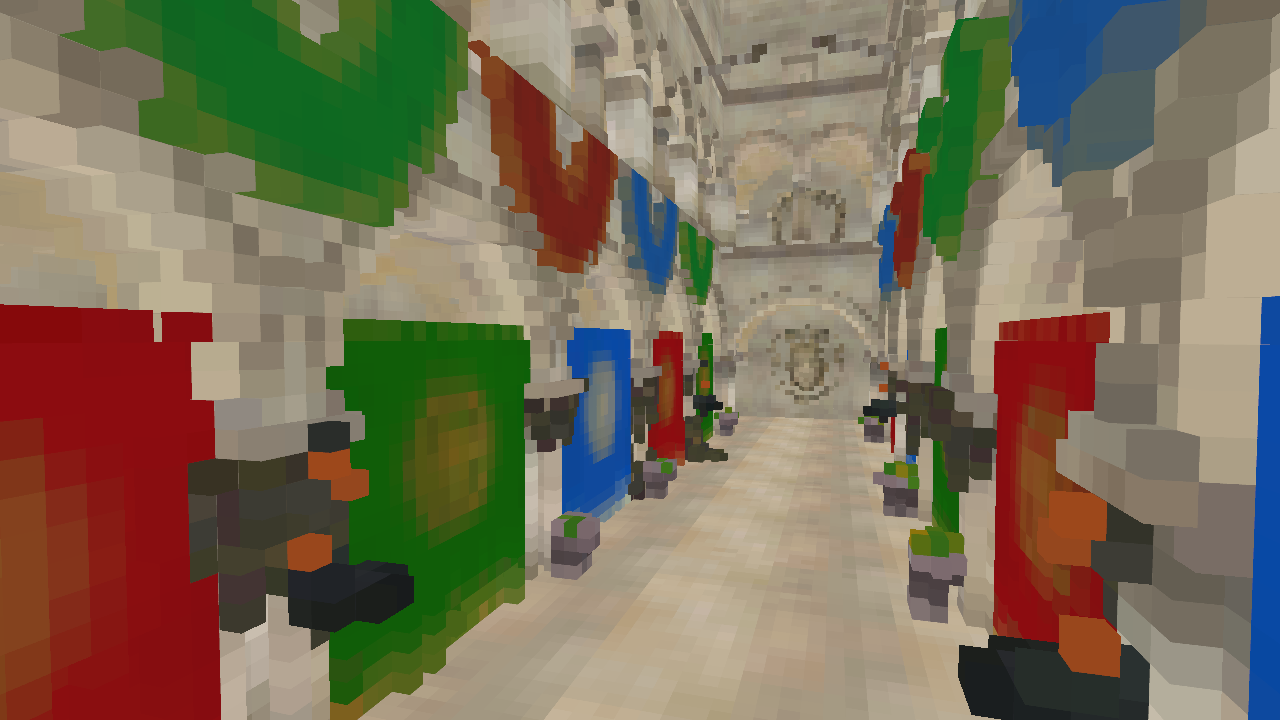
\includegraphics[width=\textwidth]{voxels_off.png}
    \caption{Visualization of the voxels resulting from the rasterization-based approach (without conservative rasterization).}
    \label{fig:voxels_off}
\end{figure}

% TODO need to work this in better. subsection?
% TODO should expand on problem more
\subsubsection{Conservative Rasterization}
As mentioned previously, we need conservative rasterization to minimize holes and cracks in the voxelization. To achieve this, we use an MSAA-based approach~\cite{takeshige2015basics}. MSAA (multi-sample anti-aliasing) is a technique used for smoothing out ragged edges (aliasing) in a rasterized image. Instead of only sampling at one position inside a pixel to determine if a fragment should be generated multiple samples are used (hence the name). These samples are typically distributed to maximize the possibility of a rasterized fragment being produced. If any of the samples overlap with the triangle a fragment is generated for that pixel. An illustration of MSAA is shown in Figure~\ref{fig:msaa}. Applied to voxelization, this means there is a smaller chance that a triangle will fail to produce a fragment for any voxel it only partially occupies. While the MSAA method of conservative rasterization is not perfect (a partially occupied voxel won't always produce a fragment), it is cross-platform, simple to use, and efficient. Other notable methods would be manually dilating each triangle in a geometry shader (better quality but slower)~\cite{akenine2005conservative} or using a GPU vendor specific extension, like \verb#GL_NV_conservative_raster# (better quality but not cross-platform). A comparison between no conservative rasterization, MSAA-based conservative rasterization, and the NVIDIA extension is shown in Figure~\ref{fig:conservativerasterization}\footnote{Also note the erroneous fragments generated when using the NVIDIA extension. These extra fragments are produced by some methods of (overly) conservative rasterization and the user must manually cull these fragments.}.

\begin{figure}[h]
    \centering
    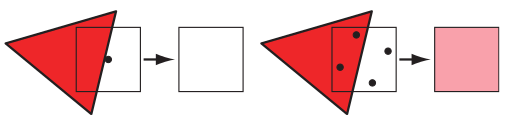
\includegraphics[width=\textwidth]{rtr_fig5_28.png}
    \caption{With MSAA, multiple points within a pixel are used to determine whether a fragment should be generated~\cite{moller2008rtr}.}
    \label{fig:msaa}
\end{figure}

% TODO should implement the geometry shader based and then compare performance quality of all 3 (might need to do that indirect rendering thing too...)

% Camera Position (8.0, 2.7, -1.3), Direction (-1.0, -0.0, 0.3)

\begin{figure}[h!]
\centering
    \begin{subfigure}[t]{0.65\textwidth}
        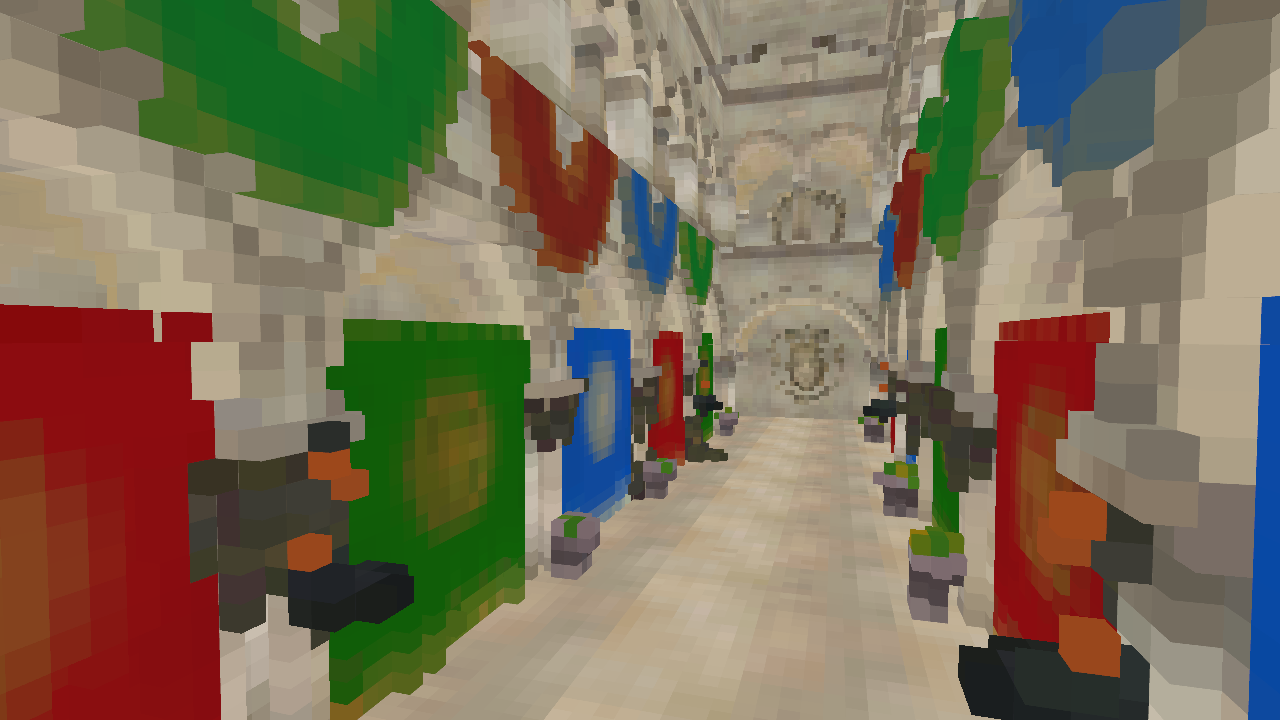
\includegraphics[width=\textwidth]{voxels_off.png}
        \caption{No conservative rasterization}
    \end{subfigure}
    \begin{subfigure}[t]{0.65\textwidth}
        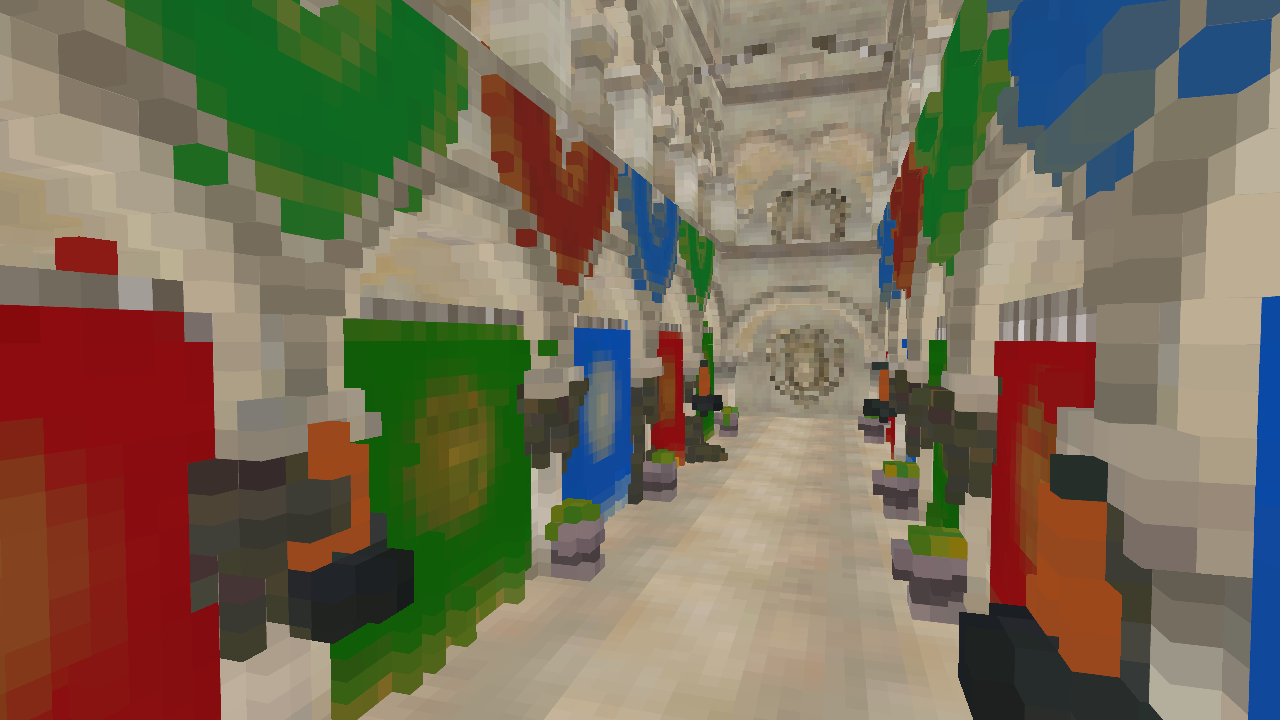
\includegraphics[width=\textwidth]{voxels_msaa.png}
        \caption{MSAA-based conservative rasterization}
    \end{subfigure}
    \begin{subfigure}[t]{0.65\textwidth}
        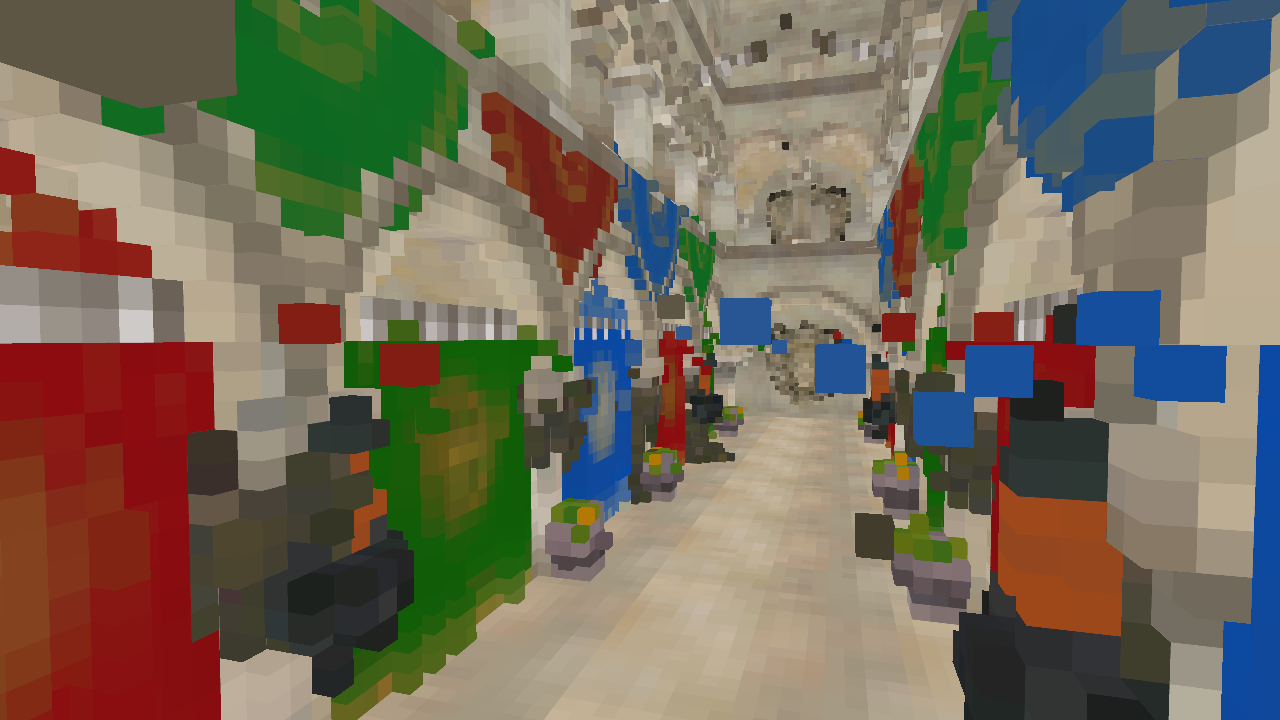
\includegraphics[width=\textwidth]{voxels_nv.png}
        \caption{NVIDIA's conservative rasterization extension}
    \end{subfigure}
    \caption{Conservative rasterization produces `extra' fragments in order to produce a more solid voxelization. The effects are particularly noticeable on the pillar between the red and green curtain on the left.}
    \label{fig:conservativerasterization}
\end{figure}

\subsection{Tessellation-Based Approach to Voxelization}
The other method for voxelization relies completely on hardware tessellation: no rasterization required. Instead of generating fragments for each voxel we instead attempt to generate vertices for each voxel. One benefit of this method is the mapping from vertex to voxel position is fairly straightforward and does not require multiple projection matrices like in the rasterization-based approach. Fei et al.~\cite{Fei:2012:PV:2305276.2305280} also developed an algorithm similar to ours using tessellation.

The core part of this approach is determining the appropriate tessellation level for a given triangle. Recall that this step is the responsibility of the tessellation control shader. Afterwards, tessellation primitive generation produces the tesselated vertices and provides them to the tessellation evaluation shader, where we compute each vertex's position in the voxel texture and store the vertex's color. The final voxelized scene is shown in Figure~\ref{fig:tesselatedvoxels}.

% TODO determining tessellation level and discarding
The desired level of tessellation will produce one vertex for each voxel the triangle covers. Therefore, for a particular triangle, the tessellation level is determined based on the triangle's size in world space. Recall that for triangular tessellation patches there are four values: three outer tessellation levels (one for each edge) and one inner tessellation level. To determine the outer tessellation level for an edge $E$, we effectively determine how many voxels $E$ passes through (accounting for the direction of $E$): $\displaystyle outerLevel = \frac{|E|}{(\frac{E}{||E||} \cdot voxelSize)}$. To determine the inner tessellation level, we find the maximum altitude of the triangle and then perform a similar computation as with the outer level. With $a$, $b$, and $c$ being the lengths of the triangle edges, the altitude from a side $x \in \{a, b, c\}$ is given by
\[
    h_x = \frac{2 \sqrt{s(s-a)(s-b)(s-c)}}{x}
\]
where $s = (a + b + c) / 2$ is the semiperimeter and the square root term is the triangle's area using Heron's Formula. The maximum altitude is then $h_{max} = \max(h_a, h_b, h_c)$. Finally, we have $innerLevel = h_{max} / voxelSize$. % TODO should find direction of h_max and do dot product like outer levels

% TODO calculating coordinates and inserting
After specifying the tessellation levels in the tessellation control shader, tessellation primitive generation produces the vertices that correspond to the voxels. In the tessellation evaluation shader the vertex position (in world space) is used to determine the final voxel position and is written out to the voxel texture.

An important consideration for this method is the maximum tessellation level supported by the hardware. For large triangles it is possible the tessellation will not produce a solid voxelization. A simple way to address this issue is to break large triangles into smaller ones when loading the mesh. Another consideration is for small triangles where all vertices occupy a single voxel. To reduce the number of writes to the voxel texture the contributions of these vertices can be consolidated in the shader into a single operation.

\begin{figure}[h!]
\centering
    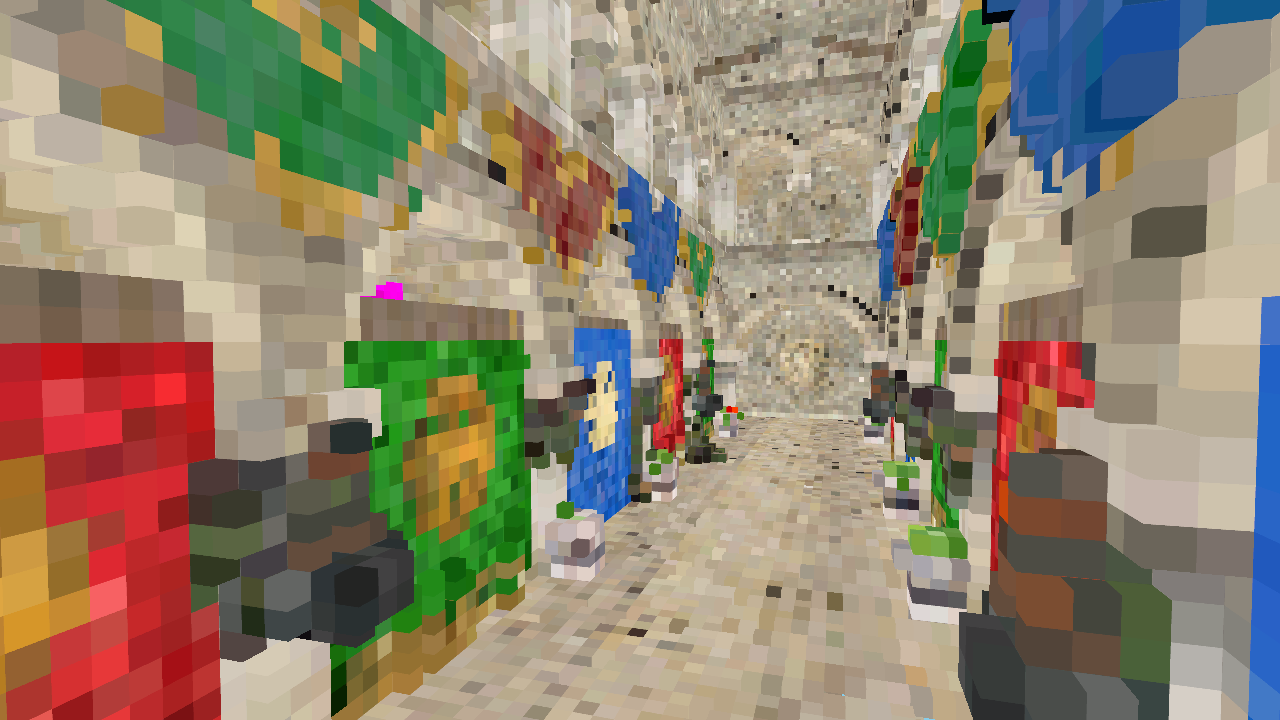
\includegraphics[width=\textwidth]{voxels_tesselated.png}
    \caption{Scene voxelized using tessellation-based voxelization.}
    \label{fig:tesselatedvoxels}
\end{figure}

% TODO code snippets, actual OpenGL names
\section{Shadow Mapping}
Shadow mapping is a well known technique used for efficiently creating shadows~\cite{Williams:1978:CCS:965139.807402}. Similar to the related works, the resulting shadow map is also treated similarly to an RSM for radiance injection.

To generate a shadow map for a light, we render the scene from the light's perspective and gather the depth values of the fragments. Since we need the GPU to write to an arbitrary texture (the shadowmap), we create a framebuffer object (FBO) and attach the texture as a depth attachment\footnote{This general technique is referred to as render-to-texture.}. The FBO does not require any color attachments, as we are only interested in the depth. The matrix used to transform vertices from world space to light space is an orthographic projection matrix multiplied with a view matrix generated from the light. This matrix is often called the light view matrix. Since the GPU will automatically write depth values, the fragment shader can be completely empty. The resulting shadow map contains floating point depth values (in the range [0, 1]) which represent the distance of each point visible to the light itself. Also note that these depth values are linear since an orthographic projection matrix is used: if a perspective projection matrix is used, the depth values scale logarithmically. Figure~\ref{fig:shadowmap} shows the contents of a shadowmap for our scene.

The only difference between generating a shadow map and a complete RSM is to also store the diffuse color and normal along with the depth values. Since our implementation stores voxel colors and normals already, a full RSM isn't necessary for injecting the VPLs into the radiance texture.

\begin{figure}[h!]
\centering
    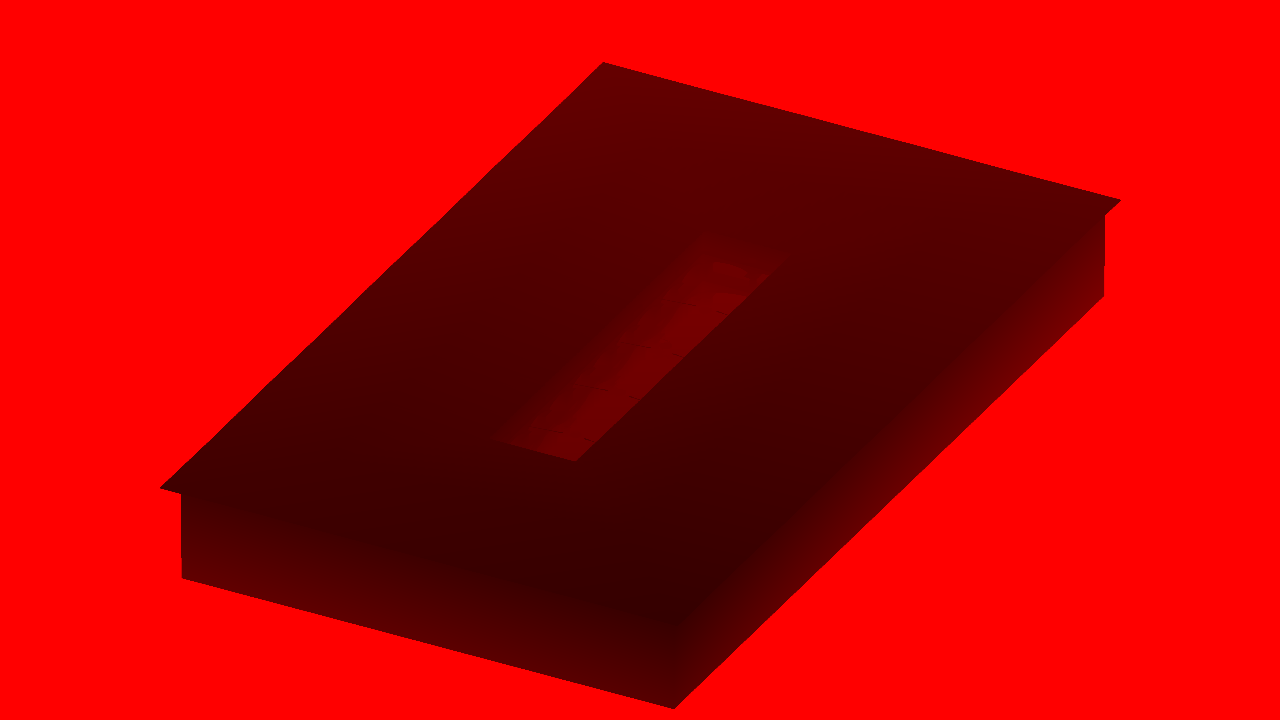
\includegraphics[width=\textwidth]{shadowmap.png}
    \caption{An example of a shadowmap with the depth value mapped to the red component of the image.}
    \label{fig:shadowmap}
\end{figure}

\section{Radiance Injection}
In this render pass, we fill a 3D texture with virtual point lights from the shadow map. Recall that the VPLs are light sources which represent the light being bounced off of geometry within the scene. Following from RSMs, the points at which this happens are precisely where the light hits the geometry, which is stored in the shadow map. Therefore, this pass involves taking all points in the shadow map and projecting the color of the corresponding geometry into the radiance texture.

The radiance texture, \texttt{voxelRadiance}, has dimensions equal to that of the other voxel textures. It has a format of \texttt{RGBA8} and stores a color value and opacity.

The most straightforward way to accomplish radiance injection from the shadow map is to use a compute shader and launch one thread for each pixel in the shadow map. Each thread first reads the depth value at its respective pixel, which can then be used to reconstruct the pixel's position in light space. Then, by using the inverse light view matrix, we project it from light space to world space. The world space position is used to calculate the voxel position, which is used to sample from the voxel textures and finally write the color into the radiance texture, as seen in Figure~\ref{fig:radiance}.

It is important that the shadowmap is rendered with a high enough resolution (relative to the voxel texture resolution) to ensure a smooth radiance injection. If the shadowmap resolution is too low, there will be gaps between voxels which cause lighting artifacts. Note also that we do not need to be concerned with synchronization and atomic operations in the case that multiple threads access the same voxel position since we are only interested in the base color.

In addition to injecting the VPLs, we also transfer occlusion information (opacity) stored in the completely voxelized scene into the radiance texture. This operation is a straightforward transfer accomplished using another compute shader.

% TODO show lighting artifacts if shadowmap resolution too low
% TODO temporal filtering?

% \begin{lstlisting}[language=C,breaklines=true,basicstyle=\footnotesize\ttfamily]
% vec2 shadowmapTexcoord = vec2(threadId) / vec2(shadowmapSize);
% float shadowmapDepth = texture(shadowmap, shadowmapTexcoord).r;
% vec3 ndc = vec3(shadowmapTexcoord, shadowmapDepth) * 2 - vec3(1);
% vec3 worldPosition = (lsInverse * vec4(ndc, 1)).xyz;
% ivec3 voxelPosition = ivec3(voxelIndex(worldPosition, voxelDim, voxelCenter, voxelMin, voxelMax, warpVoxels));
% \end{lstlisting}

\begin{algorithm}
    \caption{Radiance Injection}
    \label{alg:radianceinjection}
    \begin{algorithmic}
        \For{$\text{each pixel coordinate } p = (p_x,p_y) \text{ in shadowmap}$} \Comment{$p_x, p_y \in [0,1]$}
        \State {$depth = \mathrm{sampleDepthFromShadowmap}(p)$}
        \State {$ndc = (p_x, p_y, depth) * 2 - 1$} \Comment{Convert coordinate to NDC}
        \State {$worldPosition = inverseLight * ndc$}
        \State {$voxelPosition = \mathrm{computeVoxelPosition}(worldPosition)$}
        \EndFor
    \end{algorithmic}
\end{algorithm}

\begin{figure}[h!]
\centering
    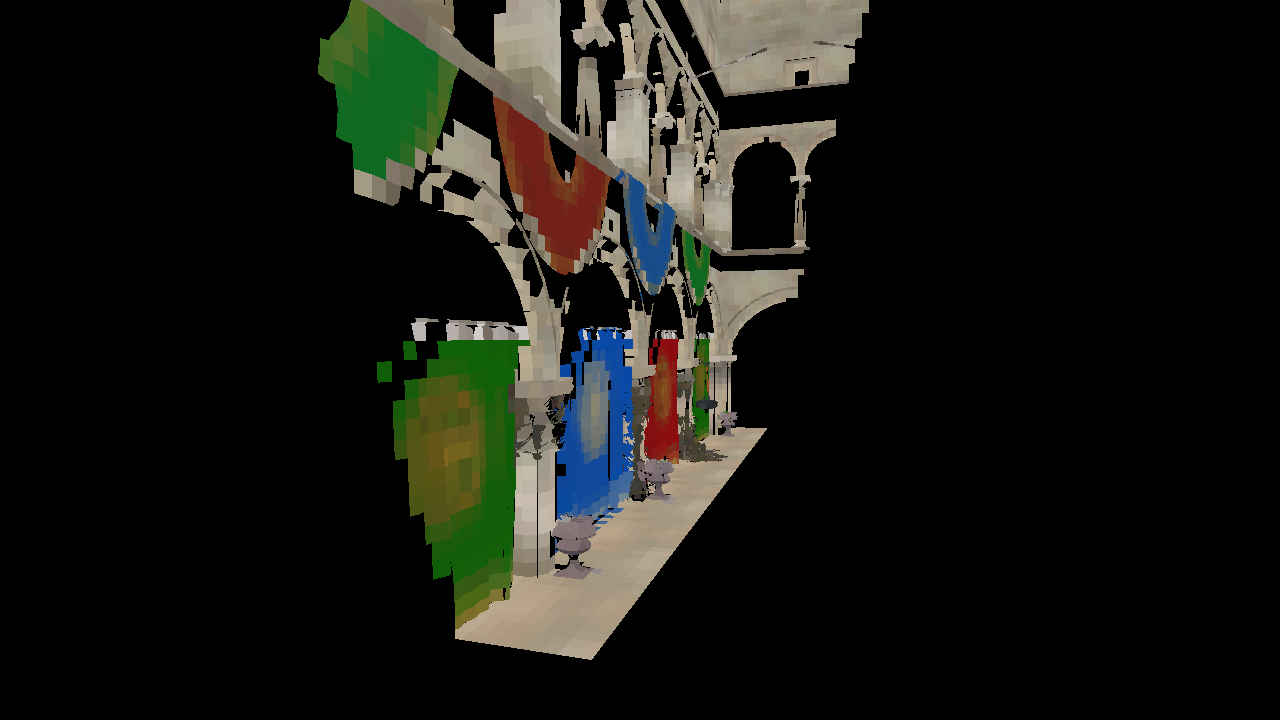
\includegraphics[width=\textwidth]{radiance_nolighting.png}
    \caption{The radiance texture injects VPLs according to the shadowmap: only voxels hit by the light source result in a VPL.}
    \label{fig:radiance}
\end{figure}

\section{Radiance Filtering}
With the highest level of detail of the radiance texture filled, the next step is creating the filtered representation. Each successive level is half the resolution of the previous level. Therefore, the maximum number of levels the texture may have is $log_2 (\max (\text{width}, \text{height})) + 1$.

% TODO timing difference between glgenmipmaps and compute shader
OpenGL is able to automatically generate mipmaps for 3D textures by calling \verb#glGenMipmaps(GL_TEXTURE_3D)#, however manually filtering the textures using a compute shader turned out to be much faster for this application (how OpenGL calculates mipmaps is implementation defined, so the performance can vary between systems and drivers). To perform the filtering, a compute shader kernel is launched for each level of the radiance texture (not including the base level). The kernel is launched with one thread for each voxel in the current level. Each thread can be conceptually located at the corners of each voxel in the previous level and average the surrounding 8 values to compute the filtered value of its respective voxel.

% TODO probably remove this, or maybe future work?
The other benefit to manually filtering is that different methods can be used. For example, adjusting the size or weights of the filtering kernel could result in different effects.

\begin{figure}[h!]
\centering
    \begin{subfigure}[t]{0.475\textwidth}
        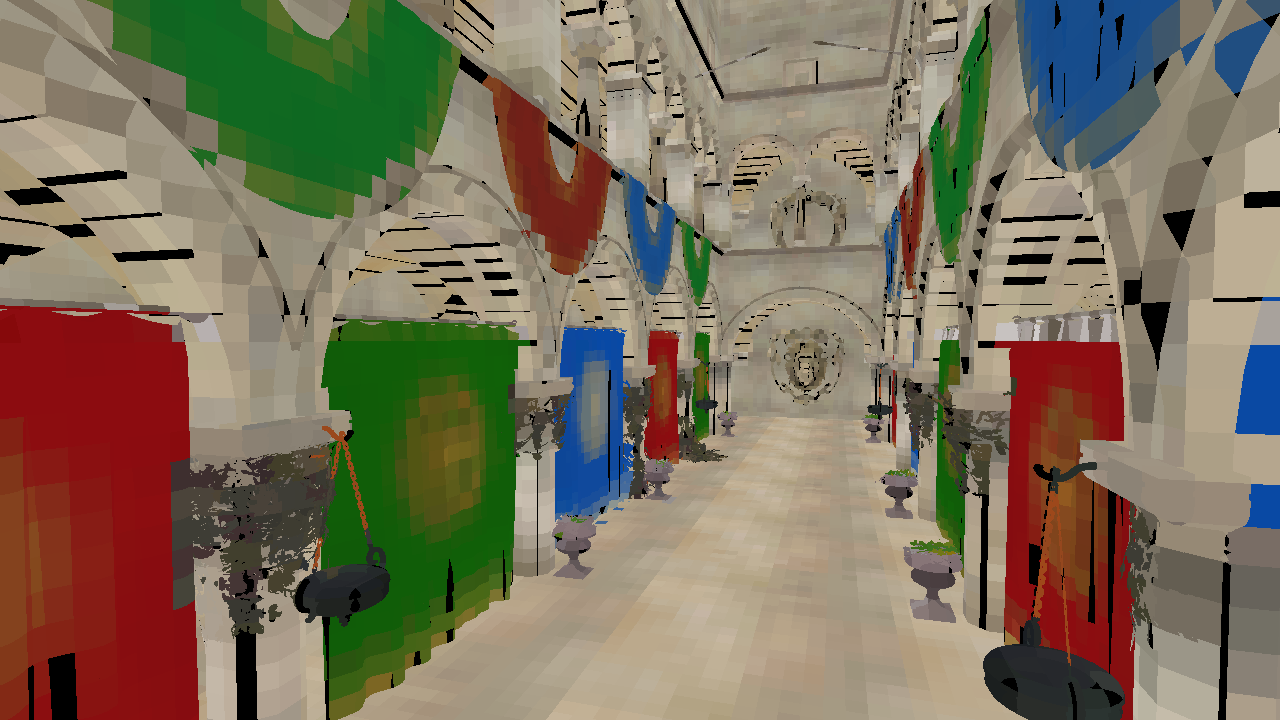
\includegraphics[width=\textwidth]{mipmap0.png}
        \caption{Level 0}
    \end{subfigure}
    ~
    \begin{subfigure}[t]{0.475\textwidth}
        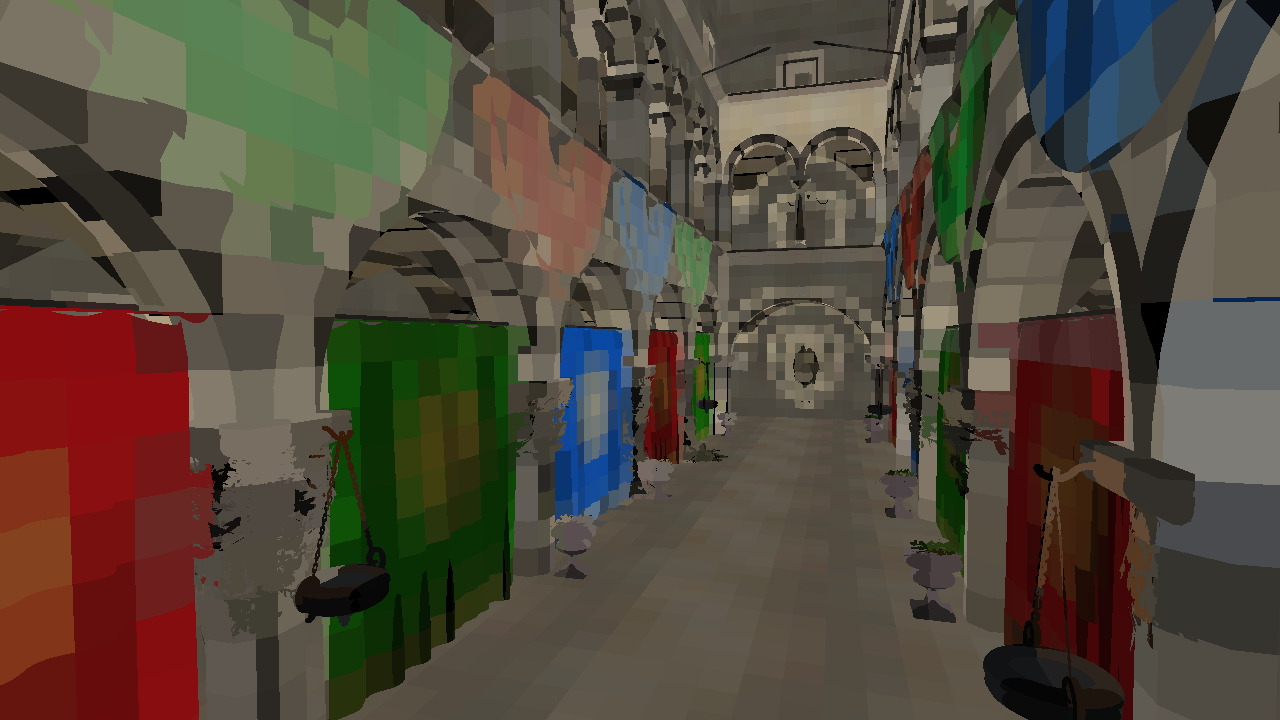
\includegraphics[width=\textwidth]{mipmap1.png}
        \caption{Level 1}
    \end{subfigure}
    \begin{subfigure}[t]{0.475\textwidth}
        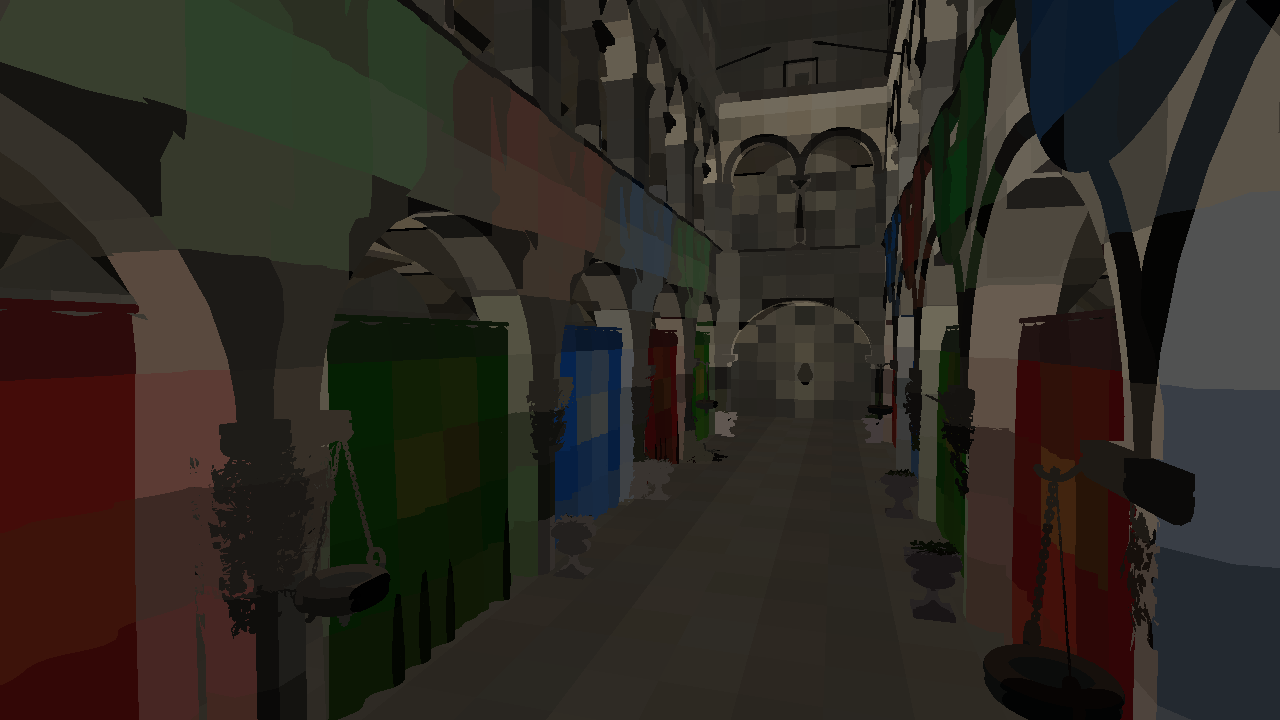
\includegraphics[width=\textwidth]{mipmap2.png}
        \caption{Level 2}
    \end{subfigure}
    ~
    \begin{subfigure}[t]{0.475\textwidth}
        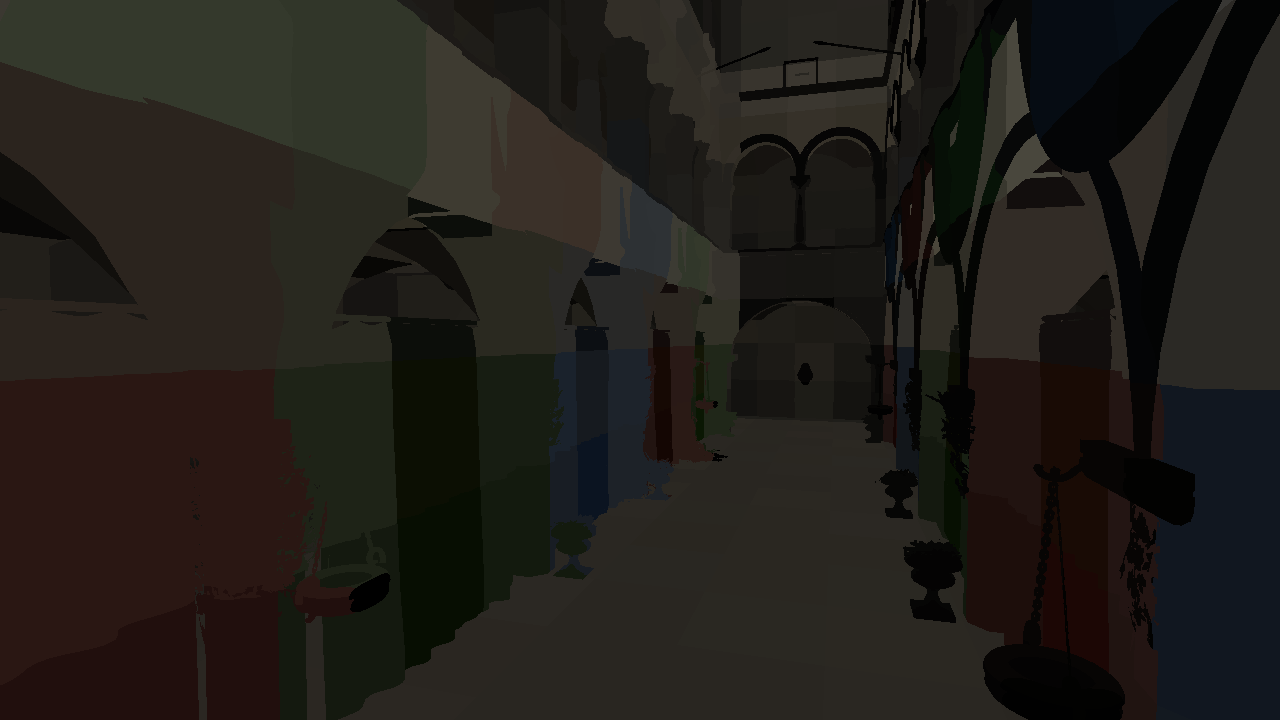
\includegraphics[width=\textwidth]{mipmap3.png}
        \caption{Level 3}
    \end{subfigure}
    \caption{The first 4 levels of the radiance texture are shown here (using \texttt{GL\_NEAREST\_MIPMAP\_NEAREST} filtering for demonstration purposes).}
    \label{fig:radiancefiltered}
\end{figure}

\section{Shading}
% TODO do i need to show code/go step by step here?
The final shading step takes all of the previously generated information and renders the scene. Direct lighting is computed from multiple lights and uses the physically based Cook-Torrance shading model~\cite{Cook:1982:RMC:357290.357293}. The classic Blinn-Phong shading model~\cite{Phong:1975:ICG:360825.360839} is also supported. Indirect lighting is computed using voxel cone tracing. Normal mapping (similar to bump mapping~\cite{Blinn:1978:SWS:965139.507101}), shadow mapping, and post processing effects also occur here. A complete outline of computing the final shaded color is shown in Algorithm~\ref{alg:finalshading}.

% TODO section  on normal mapping, shadow mapping, postprocessing?  or maybe in background?

% TODO explain UBO offsets and such? (also should this be in background?)
Two important inputs for the fragment shader are material information and light information. The material information for each fragment is provided in a struct \texttt{Material}, uploaded as a uniform buffer object, and contains color and texture information. Lights are stored as an array of struct \texttt{Light}s and contain information associated with them such as light type (e.g.\ directional or point light), position, and color. The array is uploaded as a shader storage buffer object, which allows the array to have a dynamic size queryable at shader runtime.

\begin{algorithm}
    \caption{Final Shading (performed on each rasterized fragment)}
    \label{alg:finalshading}
    \begin{algorithmic}
        \State {$directLighting = 0$}
        \For {each light in the scene}
            \State {$directLighting = directLighting + \mathrm{computeDirect}()$} \Comment{Diffuse and specular lighting}
            \If {in shadow}
                \State {$shadowFactor = \mathrm{computeShadowAmount}()$}
                \State {$directLighting = shadowFactor * directLighting$}
            \EndIf
        \EndFor
        \State {}

        \State {$indirectLighting = 0$}
        \For {each diffuse cone}
            \State {Transform cone direction to world space} \Comment{Using TBN matrix}
            \State {$color, occlusion = \mathrm{coneTrace}()$} \Comment{Perform cone tracing, resulting in a color and occlusion factor}
            \State {$indirectLighting = indirectLighting + occlusion * color$}
        \EndFor
        \State {}

        \State {$reflectedDirection = \mathrm{reflect}()$} \Comment {Compute direction of reflected ray}
        \State {$reflectColor, reflectOcclusion = \mathrm{coneTrace}()$}
        \State {$indirectLighting = indirectLighting + reflectOcclusion * reflectColor$}
        \State {}

        \State {$finalColor = directLighting + indirectLighting$}
        \State {$finalColor = finalColor / (finalColor + 1)$} \Comment{Tone map}
        \State {$finalColor = finalColor^{\frac{1}{2.2}}$} \Comment{Gamma correction}
    \end{algorithmic}
\end{algorithm}

% \missingfigure{Final rendered image with each individual contribution (direct+ diffuse indirect + specular indirect)}

\subsection{Direct Lighting}
We calculate direct lighting by iterating over each light source in the scene and summing all lighting contributions. We compute diffuse and specular lighting according to the Cook-Torrance shading model~\cite{Cook:1982:RMC:357290.357293} (without the ambient term, which is computed by the voxel cone tracing):
\[
    r = \sum_{i=0}^{n} l_{i_c} * (\bm{n} \cdot \bm{l_i}) * (d * r_d + s * r_s)
\]
where $r$ is the resulting color, $n$ is the number of lights, $l_c$ is the light color, $\bm{n}$ is the surface normal, $\bm{l}$ is the light vector, $d$ and $s$ are scaling factors, and $r_d$ and $r_s$ are the diffuse and specular components (the BRDFs). The diffuse component $r_d$ is calculated with the Lambertian model for diffuse light, which is simply $c / \pi$, where $c$ is the material's surface color. The specular component is
\[
    r_s = \frac{DGF}{\pi (\bm{n} \cdot \bm{l}) (\bm{n} \cdot \bm{v})}
\]
where $D$ is a Normal Distribution Function, $G$ is the Geometric Attenuation Fucntion, $F$ is the Fresnel term, $\bm{n}$ is the surface normal, $\bm{l}$ is the light vector, and $\bm{v}$ is the view vector. The Cook-Torrance model allows for different choices of $D$, $G$, and $F$. Our implementation uses the Trowbridge-Reitz GGX Normal Distribution Function, Smith Schlick-GGX Geometric Attenuation Function, and Schlick's approximation for the Fresnel term\footnote{These choices for $D$, $G$, and $F$ are the same as in Unreal Engine 4~\cite{karis2013real}.}:
\begin{align*}
    D(\bm{n}, \bm{h}, \alpha) &= \frac{\alpha^2}{\pi ((\bm{n} \cdot \bm{h})^2 (\alpha^2 - 1) + 1)^2} \\
    G1(\bm{n}, \bm{v}, k) &= \frac{\bm{n} \cdot \bm{v}}{(\bm{n} \cdot \bm{v}) (1 - k) + k} \\
    G(\bm{n}, \bm{v}, \bm{l}, \bm{k}) &= G1(\bm{n}, \bm{v}, k) G1(\bm{n}, \bm{l}, k) \\
    F &= F0 + (1 - F0) (1 - \cos \theta)^5 \\
\end{align*}
where $\alpha$ is material roughness, $\bm{h}$ is the half vector, $k = \frac{(\alpha + 1)^2}{8}$, $\theta$ is the angle between $\bm{h}$ and $\bm{v}$, and F0, the surface reflection at zero incidence, is 0.04 for dielectrics and the surface albedo for metals\footnote{This is not completely physically accurate but is a good and fast approximation.}.

% TODO definitely gonna want some pictures
% TODO present integral as going backwards? (want integral -> inf many rays -> break into discrete chunks w/ weights)
\subsection{Indirect Lighting (Voxel Cone Tracing)}
To compute the indirect lighting at a given point, we perform voxel cone tracing. Recall that to compute indirect light we are effectively approximating a surface integral over a hemisphere. With voxel cone tracing, this integral is reduced to summing the contributions of several cones, each of which are defined by a direction and cone angle\footnote{Note that as the cone angle approaches zero we effectively have a ray. In fact, the main difference between classic raymarching and cone tracing is the cone angle (which is used to determine which level of the filtered radiance to sample from).}. To compute the integral perfectly would require infinitely many cones. Instead, we use six cones: five for diffuse light and one for a specular highlight\footnote{The number of cones and their associated directions and angles are determined experimentally.}.

% TODO should either explain vct in related works or right here before detailing cone properties
% TODO multiple cones + directions, weights and math supporting it
% TODO FILL IN APERTURE (from vct settings) AND ANGLE
For the diffuse cones we chose an aperture of $45^\circ$ with one cone oriented in the direction of the surface normal and the others evenly distributed around the normal and tilted up at an angle of $45^\circ$. We also assign weights to each cone based on a uniform distribution. Note that in order to compute the orientation of each cone in world space we must multiply the chosen cone directions by the TBN matrix, since the cone directions are defined in tangent space. To get the final diffuse contribution, the cone tracing is performed for each cone and the values are weighted and summed appropriately.

% TODO make sure to define these somewhere
The specular cone is oriented in the direction of the reflection vector, which is calculated as $-\bm{v} - 2 * (\bm{n} \cdot -\bm{v}) * \bm{n}$, or by using the GLSL function \texttt{reflect()}. The aperture is derived from the material's roughness according to the following formula\footnote{Determined experimentally.}: $0.1 * \pi * roughness$.

% \missingfigure{Show hemisphere with the cones used}

% TODO place this somewhere...
% TODO  add math n shit yo
The radiance texture is sampled at varying levels of detail in order to approximate the amount of indirect light at that point. At it's core, voxel cone tracing is raymarching through a mipmapped texture. In order to determine which miplevel to sample from, the idea of cone tracing is introduced. Instead of having a simple ray, we imagine a cone with a particular aperture (angle). The cone's height is analagous to a ray's length and the size (diameter) of the cone's base grows as the height increases. We can then map the diameter to a level of detail.

Combining this all together, we sample from the radiance texture at a level of detail related to the height of the cone at our sampling point. In this way, samples close to the start of the cone come from higher detailed data and samples far from the start come from lower detailed data. This allows the voxel cone tracing to gather both high frequency and low frequency details of the indirect light.

% TODO go over all the vct settings
The implementation of a single cone tracing instance is done entirely within a fragment shader. The main inputs are the radiance texture, the position to start tracing from, and the direction in which to trace. There are also several configurable parameters that influence the cone tracing. We have \texttt{steps}, the maximum number of samples to take; \texttt{bias}, the initial offset from the starting position (in order to avoid self illumination); \texttt{coneAngle}, the angle of the cone; \texttt{coneHeight}, the starting height of the cone; and \texttt{lodOffset}, a constant offset used when determining the level of the radiance texture to sample from. Also, since the cone tracing is performed in texture space, a \texttt{scale} is applied to normalized direction vectors. For each step, the cone's radius is computed from the cone's height and angle. From this, we compute the level of detail to sample from. After getting the sample color and alpha value a forward blending scheme is used. Finally, the cone's height is increased for the next iteration of the loop. The complete shader code for cone tracing is shown in Listing~\ref{lst:vct}. The lighting contribution from the indirect light (both diffuse and specular) is displayed in Figure~\ref{fig:debugindirect} and the occlusion values are displayed in Figure~\ref{fig:debugocclusion}.

\begin{lstlisting}[caption={Shader function for performing voxel cone tracing.},label={lst:vct}]
vec4 traceCone(sampler3D voxelTexture, vec3 position, vec3 normal, vec3 direction, int steps, float bias, float coneAngle, float coneHeight, float lodOffset)
{
    vec3 color = vec3(0);
    float alpha = 0;

    float scale = 1.0 / voxelDim;
    vec3 start = position + bias * normal * scale;
    for (int i = 0; i < steps && alpha < 0.95; i++) {
        float coneRadius = coneHeight * tan(coneAngle / 2.0);
        float lod = log2(max(1.0, 2 * coneRadius));
        vec3 samplePosition = start + coneHeight * direction * scale;

        vec4 sampleColor = textureLod(voxelTexture, samplePosition, lod + lodOffset);
        float a = 1 - alpha;
        color += sampleColor.rgb * a;
        alpha += a * sampleColor.a;
        coneHeight += coneRadius;
    }

    return vec4(color, alpha);
}
\end{lstlisting}

% \begin{algorithm}
%     \caption{Voxel Cone Tracing}
%     \label{alg:voxelconetracing}
%     \begin{algorithmic}
%         \Procedure{TODO}{}
%         \EndProcedure
%     \end{algorithmic}
% \end{algorithm}

\begin{figure}[h!]
\centering
    \begin{subfigure}[t]{\textwidth}
        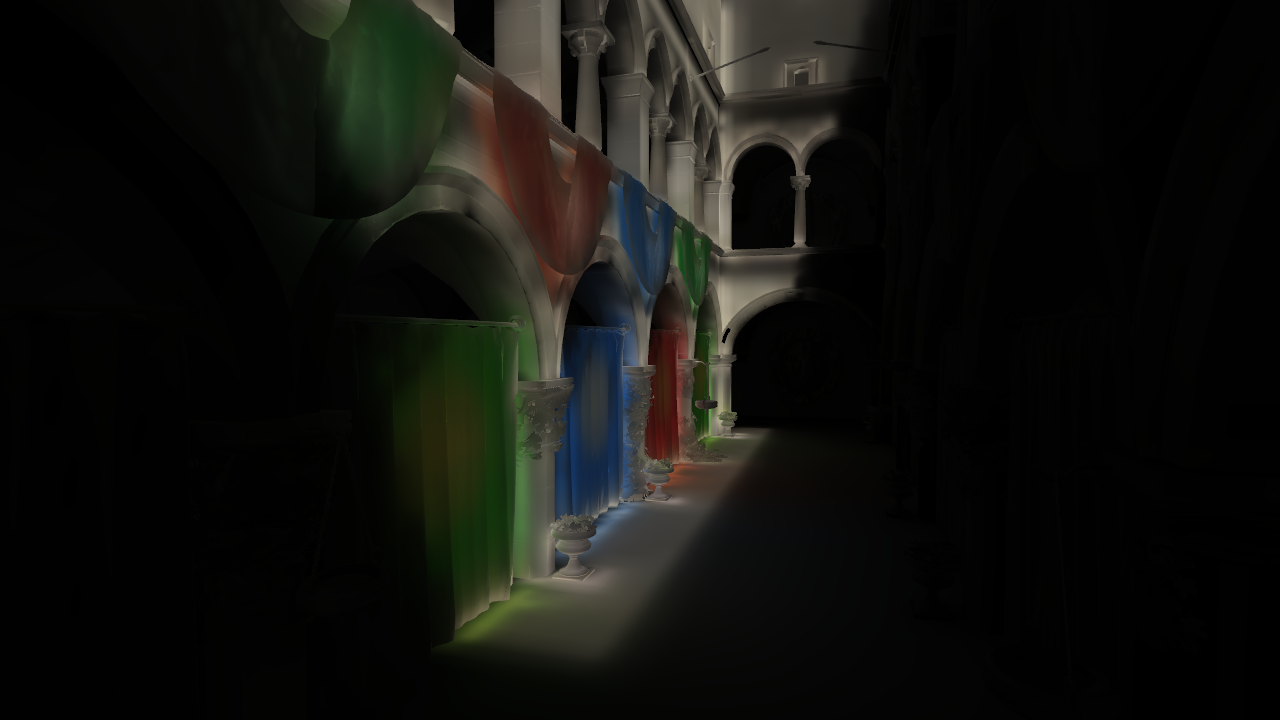
\includegraphics[width=\textwidth]{debugIndirect_noOcclusion.png}
        \caption{Diffuse indirect light}
    \end{subfigure}
    \begin{subfigure}[t]{\textwidth}
        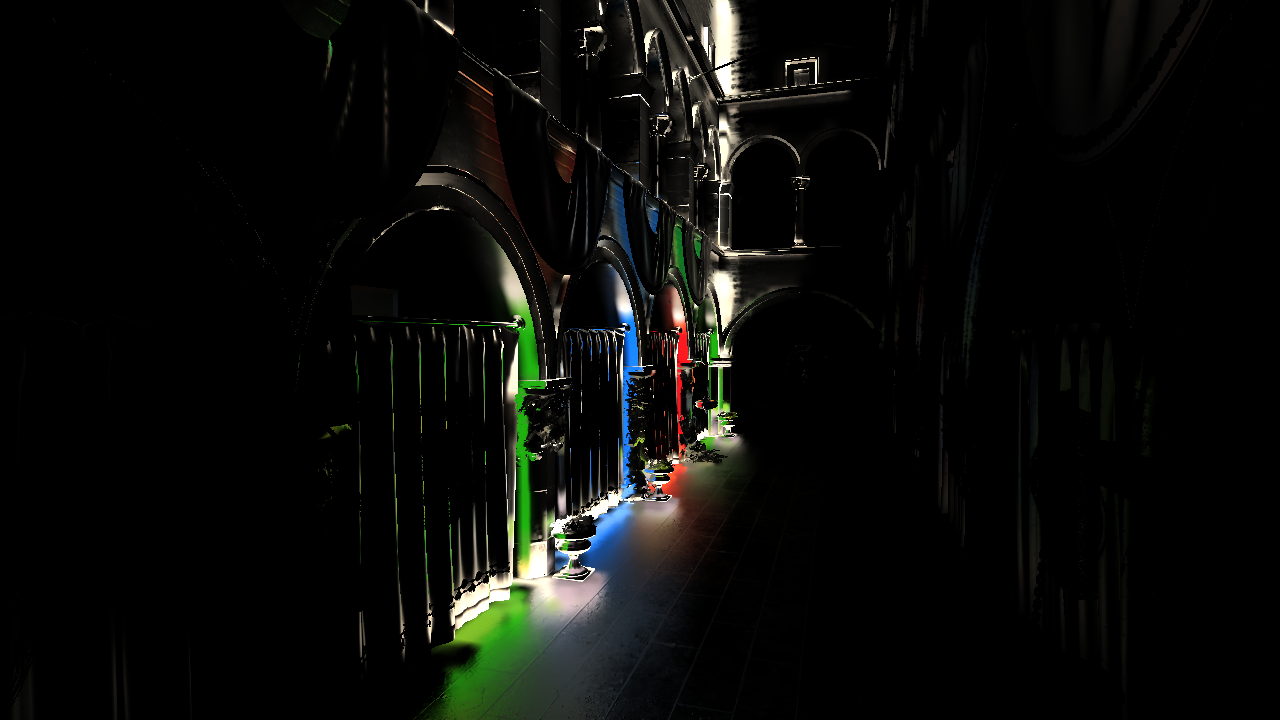
\includegraphics[width=\textwidth]{debugReflections.png}    % TODO multiplied by occlusion?
        \caption{Specular indirect light}
    \end{subfigure}
    \caption{The diffuse and specular contributions from cone tracing (before multiplying by occlusion).}
    \label{fig:debugindirect}
\end{figure}

\begin{figure}[h!]
\centering
    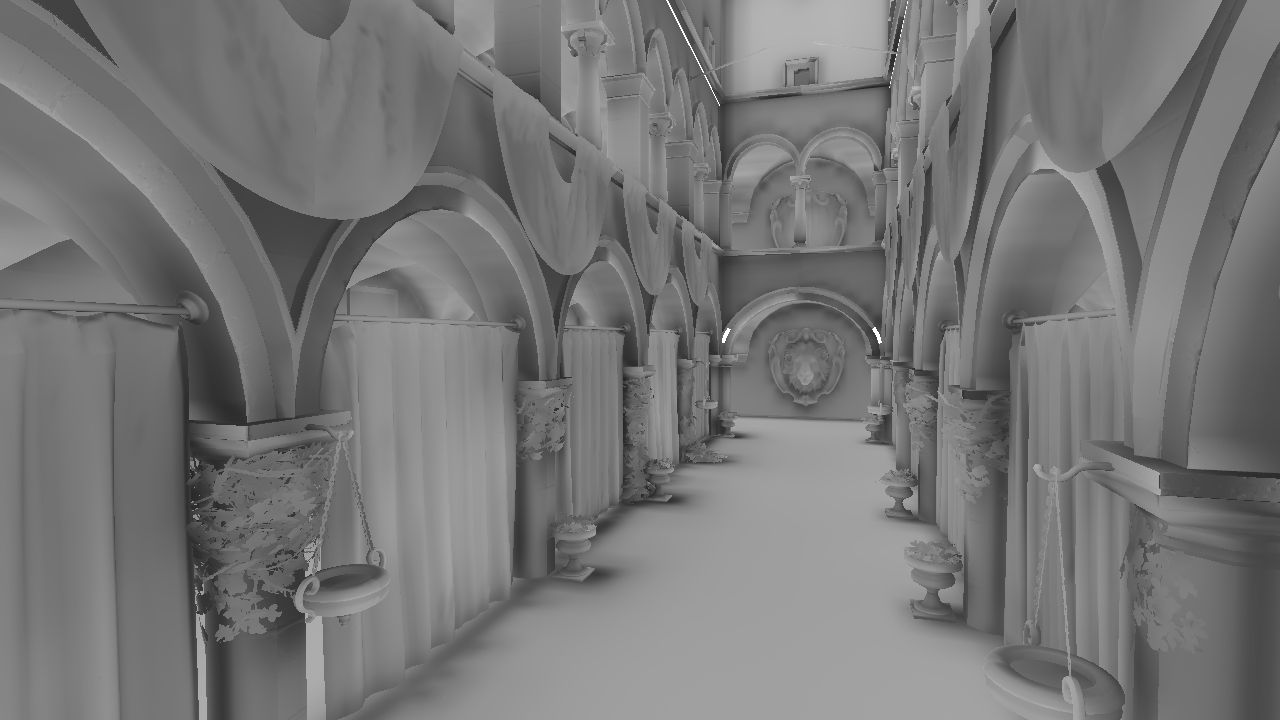
\includegraphics[width=\textwidth]{debugOcclusion.png}
    \caption{Occlusion values resulting from voxel cone tracing. The occlusion is multiplied with the cone traced lighting in order to account for occlusion of nearby objects (i.e.\ voxel based ambient occlusion).}
    \label{fig:debugocclusion}
\end{figure}

\section{Voxel Warping}
% TODO deriving spline, why need constraints, increasing viewport resolution
The goal of voxel warping is to vary the density of the voxel resolution according to some metric. This effectively increases the detail of the voxelization, leading to better global illumination. We present two different approaches for voxel warping: warp functions and perspective warping.

\subsection{Using a Warp Function}
Previously, voxel positions were determined linearly from their position inside the voxel volume to a position in the voxel texture. This approach takes that linear position and applies a mapping to it to find the final position inside the voxel texture. With an appropriate warping function, the voxel density can be modified. For this approach, the warping function's job is to increase detail near the camera and then smoothly fall off for objects further away.

\subsubsection{Linear Warp Function}
Recall from voxelization that in order to determine the location in the voxel texture for a given fragment we perform a linear mapping from world space to image space. As an intermediate step, we have the voxel position in texture space (in the range $[0, 1]$). Thus, for example, if the position along the $y$ axis is 0, it will go into the bottom of the voxel texture and if 1, it will go into the top part of the voxel texture. Now, consider mapping the coordinate in texture space to so-called warp space, which is also in the range $[0, 1]$. Without any modifications, this is a straight line with a slope of 1, representing a linear `warping' function. If we let $w_{linear}: [0, 1] \rightarrow [0, 1]$ be the warping function and $x \in [0, 1]$ be the coordinate in texture space then we have $w_{linear}(x) = x$. Of course, this warping function does not do anything useful. For that, we need a different, nonlinear, warping function.

\subsubsection{Nonlinear Warping}
Consider the function $w_{logistic}(x) = \frac{1}{1 + e^{-x}}$ (a basic logistic function, a type of ``S''-shaped curve). Notice how as $x$ approaches 0 or 1 the slope decreases and in the middle the slope is greater than one. If we draw lines up and over from the curve for $x = 0.4$ and $x = 0.6$ we see that the range of $w_{logistic}(x)$ is greater than that of $w_{linear}(x)$. In other words, the positions within those particular $x$ values `take up more space' in the voxel texture. Likewise, towards the ends, the slope decreases towards zero and thus takes up less space. This achieves the goal of varying the voxel density resolution according to a simple function. We also see that the slope, $w'(x)$, represents the voxel density: if $w'(x) = 1$, the density is the same as the linear mapping; if $w'(x) > 1$, the density is greater than the linear mapping; if $w'(x) < 1$, the density is less than the linear mapping.
% TODO lots of pictures, show  functions and lines; start off with cubic instead?

The ideal warping function increases voxel density near the camera and decreases voxel density further away. The logistic function provided does this\footnote{The camera is at the center of the voxel grid, so it corresponds to $x = 0.5$ in the warping function.}, however there are some issues. Recall from Voxelization (\autoref{sec:voxelization}) that, with the rasterized approach, the scene is rendered with a viewport of dimensions equal to that of the voxel texture. The discretized fragment positions will therefore all be in step sizes corresponding to this viewport resolution. When the warp function is applied where $w'(x) > 1$, we can run into issues where adjacent fragments will `skip' a position in the voxel texture. In essence, the voxel fragments are not generated with fine enough resolution to smoothly transition after being warped \footnote{This is similar to the concept of the Nyquist Frequency, where we are not sampling the signal at a high enough rate}. To resolve this, the scene must be voxelized with a viewport resolution scaled by the maximum derivative of $w(x)$. In design terms, this means choosing a warping function with a steep slope will result in needing to voxelize the scene with a larger viewport resolution, which can hurt performance. Figure~\ref{fig:voxelcracks} demonstrates this issue.

\begin{figure}[h!]
    \centering
    \begin{subfigure}[t]{0.475\textwidth}
        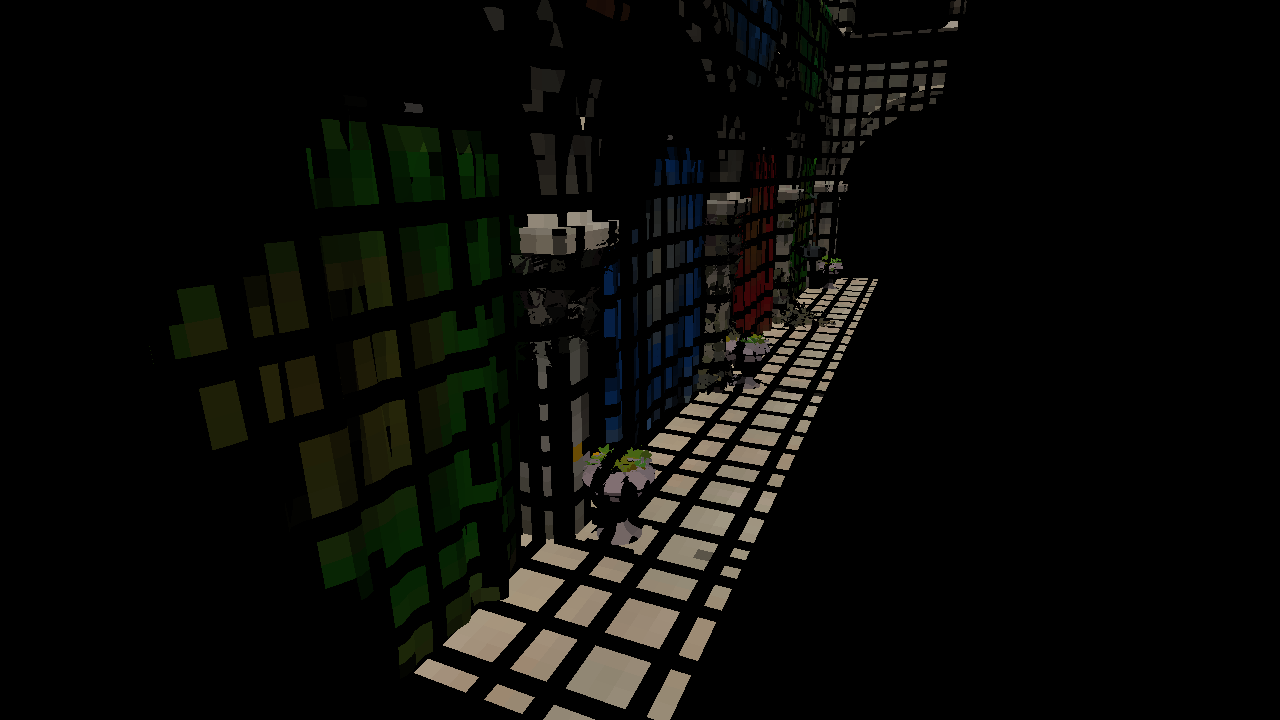
\includegraphics[width=\textwidth]{voxelwarp_cracks.png}
    \end{subfigure}
    ~
    \begin{subfigure}[t]{0.475\textwidth}
        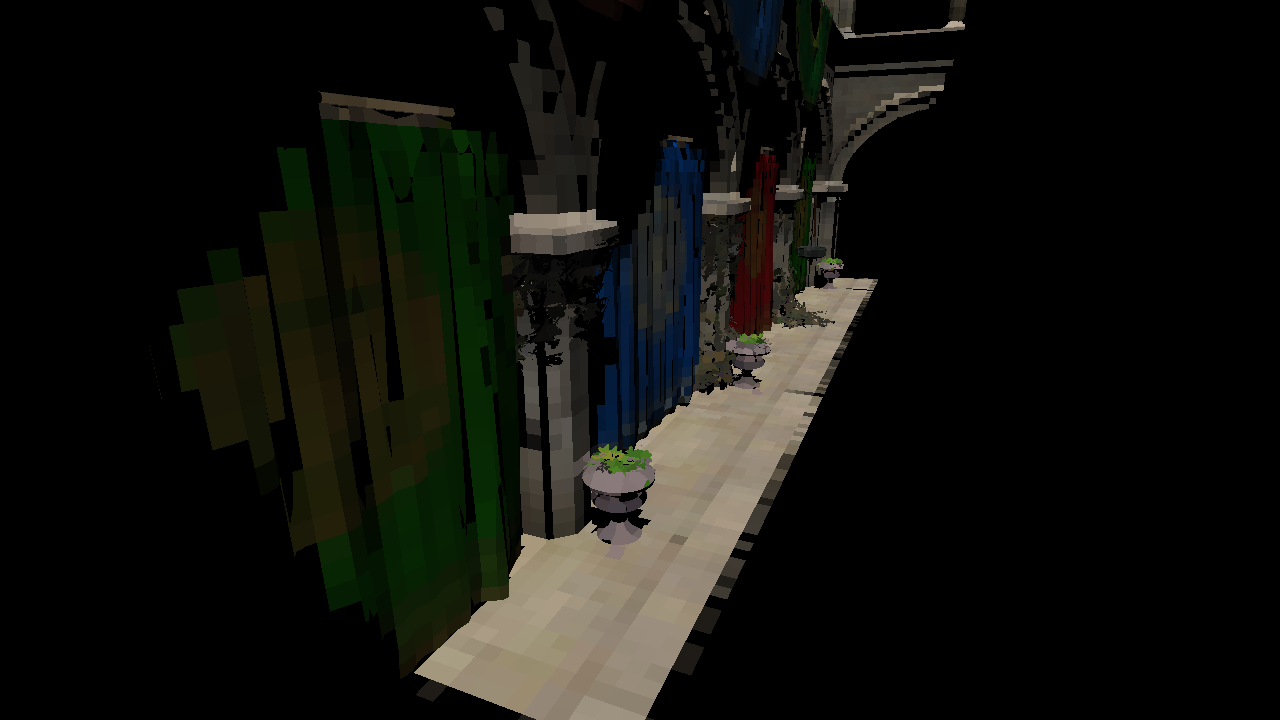
\includegraphics[width=\textwidth]{voxelwarp_nocracks.png}
    \end{subfigure}
    \caption{Cracks in the voxels caused by higher voxel density (left) and filling the holes by voxelizing with a higher resolution (right).}
    \label{fig:voxelcracks}
\end{figure}

Using the logistic function as the warping function also has another issue: the slope at the ends approaches zero. This leads to a large portion of the voxelized region ending up in relatively few voxels, which diminishes the accuracy of the voxelization greatly. % TODO show this
Instead, we want to place a lower bound on $w'(x)$. The solution to this is to use a cubic spline, i.e.\ $w(x) = a + bx + cx^2 + dx^3$. Then, with $\alpha$ as the desired end slope, we use the constraints $w(0) = 0, w(1) = 1, \text{ and } w'(0) = w'(1) = \alpha$ and solve for the variables $a$, $b$, $c$, and $d$. This gives the warping function: $w(x) = \alpha x + (3 - 3 \alpha) x^2 + (2 \alpha - 2) x^3$. For our implementation, $\alpha = 0.25$.

% TODO imply that 0.5 is close to camera? idk
% TODO go over how this doesnt mess up voxel cone tracing or filtering and stuff
% TODO horner's method?

% \subsection{Warp Textures}  % TODO ???

\subsection{Perspective Warping}
The other method of warping implemented is based on perspective projection. Recall that when transforming coordinates from view space to clip space we use a projection matrix. To emulate the visual effect of distant objects appearing smaller, a perspective projection matrix applies a scaling factor to any transformed position coordinate. This scaling effectively causes distant objects to occupy less area in screen space in the final rendered image. Similarly, for our perspective warping, we use a perspective matrix to manipulate the final voxel position.

To determine the voxel position from a position in world space, we apply both a perspective projection and view matrix. This results in a point in NDC corresponding to its position within the view frustum\footnote{We also must linearize the depth (z) component of the position, as a perspective projection causes the depth to be logarithmic.}. This value is then shifted and scaled to be in texture space, which is the voxel position.

A visualization of the voxels resulting from perspective warping is shown in Figure~\ref{fig:perspectivewarping}. The view frustum is divided into voxels where voxels closer to the camera end up being smaller and those further away are bigger.

\begin{figure}
\centering
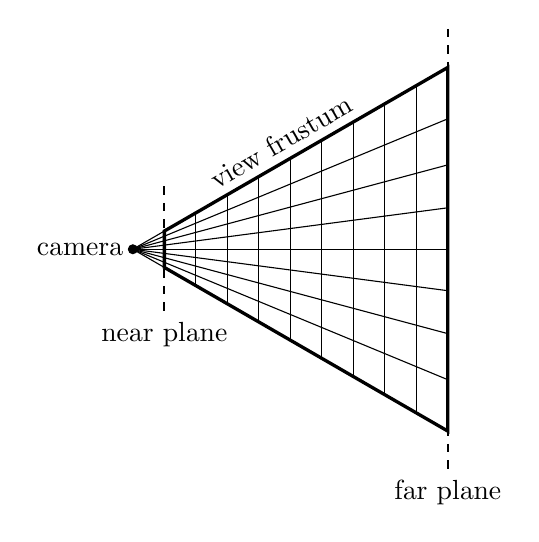
\begin{tikzpicture}[scale=0.8]
    \foreach \angle in {30, 22.5, 15, 7.5, 0, -7.5, -15, -22.5, -30} {
    \draw (0, 0) -- (5, {5 * tan(\angle)});
    }
    \foreach \z in {0.5, 1.0,...,5.0} {
    \draw (\z, {\z * tan(30)}) -- (\z, {\z * tan(-30)});
    }
    \filldraw (0,0) circle (2pt) node[anchor=east] {camera};
    \draw[dashed, thick] (0.5, 1) -- (0.5, -1) node[anchor=north] {near plane};
    \draw[dashed, thick] (5, 3.5) -- (5, -3.5) node[anchor=north] {far plane};
    \draw[very thick] (0.5, {0.5 * tan(30)}) -- (5, {5 * tan(30)}) -- (5, {-5 * tan(30)}) -- (0.5, {-0.5 * tan(30)}) -- cycle;
    \draw (2.5, {2.5 * tan(30)}) node[anchor=south, rotate=30] {view frustum};
\end{tikzpicture}
\caption{Diagram of the voxels resulting from perspective warping.}
\label{fig:perspectivewarping}
\end{figure}

% TODO do i need this?
\section{Miscellaneous}
\subsection{Depth Prepass}
With voxel cone tracing, each fragment shader invocation is quite expensive. If we have overlapping objects in the scene then fragments will be shaded for each pixel, but only one will be the final color. To ensure we only shade the final fragment, we have a prepass which rasterizes the scene and only writes the depth value. This operation is extremely quick. Now, the depth buffer contains only the depth of the fragment that will end up on the screen. When the full shading pass is performed all fragments that fail the depth test can be immediately discarded, avoiding the expensive voxel cone tracing\footnote{This technique is only needed for a forward rendering engine: for a deferred rendering engine the final depth values are calculated when generating the G-buffer (geometry buffer).}.
% TODO give before/after improvement

% \subsection{Compressed Textures with Pregenerated Mipmaps}
% TODO ?

\subsection{Temporal Filtering}     % TODO ???
Typically the radiance texture is cleared completely at the beginning of each frame. Due to the discrete nature of the voxel grid, moving objects and lights can cause temporal artifacts (flickering) as the voxels are updated. These artifacts can be improved by incorporating previous radiance values into the current frame's radiance. To do this, we can blend some factor of a voxel's previous radiance value with its new value\footnote{This factor is configurable at runtime.}.

% \subsection{Voxel Hole Filling}     % TODO ??? (radianceDilate,voxelizeDilate,voxelFillHoles)


% TODO custom filtering, try raymarching optimizations from nvidia blog
\chapter{Results and Discussion}

Here we examine both the performance and visual quality of our global illumination algorithm. The primary means of evaluating performance is based on frame time. The times of each render pass are recorded as well as a total frame time. Evaluating visual quality is based largely on whether the lighting appears smooth and believable with a minimal amount of noise and artifacts.

We also discuss the application of voxel warping and how it compares with other global illumination methods. Unfortunately, direct performance and visual quality comparisons are difficult to objectively measure as there are many contributing factors---mesh complexity and optimizations, texture resolution and format, shading model, graphics API, hardware, GPU driver version, and more---that affect the final comparison, in addition to the exact implementation details. Nevertheless, we provide motivations and tradeoffs between our method and others and their potential impact on performance and quality.

\section{Test Setup}
% TODO verify driver, kernel, resolution when getting final results
All results are obtained from a system with an i5-2400 CPU, 8GB of DDR3 RAM, and an NVIDIA GeForce GTX 970 GPU. The system is running Arch Linux kernel 4.16.8-1 and uses the proprietary NVIDIA graphics driver version 396.24. The application uses an OpenGL 4.5 context and the scene is rendered with a window resolution of 1920x1080.

% TODO give #vertices, texture resolutions and sizes?
The model used in the test scenes is the Crytek Sponza scene\footnote{The original Sponza model can be acquired from Crytek~\cite{sponza_og}. The model we use is modified by Alexandre Pestana~\cite{sponza_pbr}.}. The textures from the original Sponza scene are replaced with ones necessary for physically-based rendering (materials are defined by a diffuse color, roughness, metallic coefficient, normal, and optionally an alpha texture). Mipmaps for the original textures were also precomputed and stored along with the full size 1024x1024 textures as DDS (Microsoft DirectDraw Surface) files using the compressed DXT5 format for faster scene loading.

To measure performance timings for each render pass we make use of OpenGL timer queries using the \verb#GL_TIME_ELAPSED# query type. The results of the query object are double buffered to ensure introducing the timer query does not affect the total render time.

Unless otherwise mentioned, voxel resolutions are 256x256x256 with 6 mipmap levels.

\section{Analysis}
In the following sections we evaluate various aspects of our work. First, we discuss the global illumination algorithm as a whole. Second, we compare the rasterization-based and tessellation-based voxelization algorithms. Lastly, we provide the results of our voxel warping and some insights on future improvements.

\subsection{Global Illumination}
We test the algorithm with different screen resolutions and voxel grid resolutions. The rendered images with different voxel grid resolutions are shown in Figure~\ref{fig:results_rendered}. We see that the main difference with different voxel grid resolutions is how far the light spreads due to the larger voxels.

Table~\ref{tbl:renderpasstiming} shows timing results from the complete global illumination algorithm and Figure~\ref{fig:renderpasstiming} plots the data as a stacked bar chart. Recall that a minimum goal for real-time is 30 frames per second and a target is 60 frames per second, which correspond to individual frame times of 33.3ms and 16.7ms, respectively. We see that the total frame time always meets the goal of 60 frames per second.

The data shows that shadowmap creation and radiance injection was independent of screen resolution and voxel resolution\footnote{As expected, since the main factor for both of these render passes is the size of the shadowmap, which remained constant at 4096x4096.}. The voxelization and radiance filtering steps both only depended on voxel grid resolution. The depth prepass also only varied with respect to screen resolution. The final shading predictably depended on both voxel grid resolution and screen resolution. However, larger voxel grid resolutions did not affect the final shading times by much at a given screen resolution, with approximately a 1.5ms difference between using a voxel resolution of 64 versus 256. Ultimately, the time spent for the shading dominates all other render passes and thus makes itself a prime target for any future work on optimizing for speed.

\begin{figure}
\centering
\begin{subfigure}[t]{0.475\textwidth}
    \adjincludegraphics[width=0.95\textwidth,trim={0 {0.1\height} {0.25\width} 0},clip]{results_720_64}
    \caption{}
\end{subfigure}
~
\begin{subfigure}[t]{0.475\textwidth}
    \adjincludegraphics[width=0.95\textwidth,trim={0 {0.1\height} {0.25\width} 0},clip]{results_720_128}
    \caption{}
\end{subfigure}

\begin{subfigure}[t]{0.475\textwidth}
    \adjincludegraphics[width=0.95\textwidth,trim={0 {0.1\height} {0.25\width} 0},clip]{results_720_256}
    \caption{}
\end{subfigure}
\caption{The scene rendered with voxel grid resolutions of $64^3$, $128^3$, and $256^3$.}
\label{fig:results_rendered}
\end{figure}

\begin{table}
\centering
\small
\begin{tabular}{l ccc ccc ccc}
\toprule
Render Pass & \multicolumn{9}{c}{Render Pass Time (ms)} \\
& \multicolumn{3}{c}{1280x720} & \multicolumn{3}{c}{1600x900} & \multicolumn{3}{c}{1920x1080} \\
& 64 & 128 & 256 & 64 & 128 & 256 & 64 & 128 & 256 \\
\midrule
Voxelize           & 0.90 & 1.13 & 2.40  & 0.70 & 1.12 & 2.39  & 0.72 & 1.15 & 2.41\\
Shadowmap          & 0.69 & 0.69 & 0.69  & 0.69 & 0.69 & 0.69  & 0.68 & 0.68 & 0.69\\
Radiance Injection & 0.92 & 0.92 & 0.93  & 0.92 & 0.92 & 0.93  & 0.92 & 0.92 & 0.93\\
Radiance Filtering & 0.04 & 0.10 & 0.55  & 0.05 & 0.10 & 0.56  & 0.04 & 0.10 & 0.55\\
Depth Prepass      & 0.20 & 0.20 & 0.20  & 0.25 & 0.26 & 0.25  & 0.31 & 0.31 & 0.36\\
Final Shading      & 3.89 & 4.81 & 5.32  & 5.98 & 6.42 & 7.10  & 8.23 & 9.40 & 9.75\\
\midrule
Total              & 7.02 & 8.21 & 11.12  & 9.46 & 10.15 & 13.43  & 11.23 & 12.83 & 16.31\\
\bottomrule
\end{tabular}
\caption{Times measured for each render pass for various screen resolutions and voxel grid resolutions. The total timer also accounts for any other operations performed within each frame (i.e.\ the sum of the render pass times is not necessarily the complete time for an entire frame). Voxelization is done using the tessellation-based approach.}
\label{tbl:renderpasstiming}
\end{table}

\begin{figure}
\centering
\pgfplotstableread[row sep=\\]{
    Resolution Voxelize Shadowmap Inject Filter Shading Other\\
    720p64 0.90  0.69  0.92  0.04  4.19 0.38\\
    720p128 1.13  0.69  0.92  0.10  5.01 0.36\\
    720p256 2.40  0.69  0.93  0.55  5.52 1.03\\
    900p64 0.70  0.69  0.92  0.05  6.23 0.87\\
    900p128 1.12  0.69  0.92  0.10  6.68 0.64\\
    900p256 2.39  0.69  0.93  0.56  7.35 1.51\\
    1080p64 0.72  0.68  0.92  0.04  8.54 0.33\\
    1080p128 1.15  0.68  0.92  0.10  9.71 0.27\\
    1080p256 2.41  0.69  0.93  0.55  10.01 1.62\\
}\dataset
\begin{tikzpicture}[scale=0.9]
    \begin{axis}[nodes near coords ybar stacked configuration/.style={},ybar stacked, symbolic x coords={720p64, 720p128, 720p256, 900p64, 900p128, 900p256, 1080p64, 1080p128, 1080p256}, xtick=data, xticklabel style={rotate=45}, legend style={at={(1.05,0.5)}, anchor=west}, xlabel={Screen Resolution x Voxel Grid Size}, ylabel={Time (ms)}, enlarge y limits={0.2, upper}, title={Frame Times}, ymin=0, xlabel near ticks, xmajorticks=false]
    \addplot table[meta=Resolution, y=Voxelize] \dataset;
    \addplot table[meta=Resolution, y=Shadowmap] \dataset;
    \addplot table[meta=Resolution, y=Inject] \dataset;
    \addplot table[meta=Resolution, y=Filter] \dataset;
    \addplot table[meta=Resolution, y=Shading] \dataset;
    \addplot[point meta=y, nodes near coords, nodes near coords align={above}, nodes near coords style={/pgf/number format/.cd, fixed zerofill, precision=1}] table[meta=Resolution, y=Other] \dataset;

    \legend{Voxelize, Shadowmap, Radiance Injection, Radiance Filtering, Final Shading, Other}
    \end{axis}
\end{tikzpicture}
\caption{Graph showing the render pass times. Each bar shows the relative time contributions of each render pass. The depth prepass is incorporated into the Final Shading category and the Other category accounts for any other miscellaneous tasks done while rendering the frame.}
\label{fig:renderpasstiming}
\end{figure}

\subsection{Tessellated Voxelization}
The result of shading the scene with both voxelization methods is shown in Figure~\ref{fig:voxelcomparison}. First, we notice the rasterized approach generates `smoother' voxels. This is a result of the rasterization discretizing the fragments as well as possibly not generating fragments for small triangles. The tessellated approach, since it uses the raw vertex positions to compute the voxel position, does not exhibit this smoothing effect. Also, with the rasterized approach we see cracks on the archs from imperfect conservative rasterization. The tessellated approach does not have issues with conservative rasterization. Instead, the issue is with large triangles (such as the floor): the GPU has a maximum supported tessellation level. Triangles that require a higher tessellation level than this hardware maximum will end up having holes\footnote{A possible workaround for this would be to subdivide large triangles before voxelizing, such as when loading in the mesh.}.

In terms of both performance and visual quality both voxelization methods are very similar. Voxelization times for each method are shown in Table~\ref{tbl:voxelizationtiming} and graphed in Figure~\ref{fig:voxelizationtiming}, where we see the tessellation-based voxelization is slightly slower than the rasterization-based approach\footnote{However both implementations were not heavily optimized.}. Figure~\ref{fig:results_voxelization} compares the final rendered scene with both voxelization methods. The differences are minor.

Another limitation specific to the rasterized approach is shown in Figure~\ref{fig:voxellimitations}. The fragment resolution must be set appropriately for the voxel density\footnote{This is especially important for the warped voxelization approaches, since the density is not uniform}. The tessellated voxels do not suffer from this issue since we do not rely on the rasterizer to produce fragments.

Ultimately, both voxelization methods are sufficient for real-time global illumination. The (unoptimized) tessellation-based approach is slightly easier to implement and debug\footnote{Since the voxels are written in the tessellation evaluation stage, it is simple to add a geometry shader that takes the vertices and expands them into cubes, which are then rasterized and shaded with the vertex color (the same color inserted into the voxel texture).} but is slower than the rasterization-based approach. % One benefit of the tessellation-based approach is the voxel positions are continuous, unlike the rasterized voxels which are fixed at discrete positions according to the viewport resolution. This eliminates having to deal with cracks caused by higher density areas. (instead the limitation is on # of tesslevels ...)

\begin{figure}
\begin{subfigure}[t]{0.475\textwidth}
    \adjincludegraphics[width=\textwidth,trim={0 0 {0.25\width} 0},clip]{rastervoxel_nowarp}
    \caption{Rasterized voxels}
\end{subfigure}
~
\begin{subfigure}[t]{0.475\textwidth}
    \adjincludegraphics[width=\textwidth,trim={0 0 {0.25\width} 0},clip]{tessvoxels_nowarp}
    \caption{Tessellated voxels}
\end{subfigure}
\caption{Comparison between the scene shaded based on the rasterized voxels (left) and the tessellated voxels (right).}
\label{fig:voxelcomparison}
\end{figure}

\begin{figure}
\centering
\begin{subfigure}[t]{0.475\textwidth}
    \adjincludegraphics[width=\textwidth,trim={0 0 {0.25\width} 0},clip]{rasterlimited}
    % \caption{Rasterized voxels}
\end{subfigure}
% ~
% \begin{subfigure}[t]{0.475\textwidth}
%     \adjincludegraphics[width=\textwidth,trim={0 0 {0.25\width} 0},clip]{tesslimited}
%     \caption{Tessellated voxels}
% \end{subfigure}
% \caption{Images showing the main limitations of each voxelization method. For the rasterized approach (left), the fragment resolution must be large enough for a particular voxel density. For the tessellated approach (right), cracks appear if a higher tessellation level than the hardware supported maximum is required.}
\caption{Image showing a limitation of the rasterized approach: the fragment resolution must be large enough for a particular voxel density. Otherwise, cracks will occur in the final voxelization.}
\label{fig:voxellimitations}
\end{figure}

\begin{figure}[h!]
\centering
    \begin{subfigure}[t]{0.475\textwidth}
        \adjincludegraphics[width=\textwidth,trim={0 0 {0.25\width} 0},clip]{results_voxelraster}
        \caption{Rasterized voxels}
    \end{subfigure}
    ~
    \begin{subfigure}[t]{0.475\textwidth}
        \adjincludegraphics[width=\textwidth,trim={0 0 {0.25\width} 0},clip]{results_voxeltess}
        \caption{Tessellated voxels}
    \end{subfigure}
    \caption{The final rendered image for both voxelization methods have negligable visual differences.}
    \label{fig:results_voxelization}
\end{figure}

\begin{figure}
\centering
\pgfplotstableread[row sep=\\]{
    Resolution Rasterized Tessellated\\
    64         0.53       0.70\\
    128        0.85       1.12\\
    256        1.91       2.35\\
}\dataset
\begin{tikzpicture}[scale=0.9]
    \begin{axis}[ybar=5pt, symbolic x coords={64,128,256}, xtick=data, legend style={at={(1.05,0.5)}, anchor=west}, xlabel={Voxel Grid Size}, ylabel={Time (ms)}, enlarge y limits={0.2, upper}, enlarge x limits={0.2}, title={Voxelization Time},nodes near coords, nodes near coords align={above}, nodes near coords style={/pgf/number format/fixed}, ymin=0, ybar=10pt, xtick align=inside, xmajorticks=false]
    \addplot table[meta=Resolution, y=Rasterized] \dataset;
    \addplot table[meta=Resolution, y=Tessellated] \dataset;

    \legend{Rasterized, Tessellated}
    \end{axis}
\end{tikzpicture}
\caption{Graph comparing the voxelization time for both approaches at different voxel grid sizes.}
\label{fig:voxelizationtiming}
\end{figure}

\begin{table}[H]
\centering
\small
\begin{tabular}{lcc}
\toprule
\multirow{2}{*}{Voxel Grid Size} & \multicolumn{2}{c}{Voxelization Time (ms)} \\
& Rasterization-Based & Tessellation-Based \\
\midrule
64x64x64        & 0.53 & 0.70\\
128x128x128     & 0.85 & 1.12\\
256x256x256     & 1.91 & 2.35\\
\bottomrule
\end{tabular}
\caption{Time spent voxelizing the scene with varying voxel grid resolutions. For the rasterization-based approach the MSAA method of conservative rasterization is used.}
\label{tbl:voxelizationtiming}
\end{table}

\subsection{Integration of Voxel Cone Tracing into Existing Engines}
Voxel cone tracing is an attractive method for adding full global illumination to existing engines. The necessary information needed for the algorithm should already be available in most engines. A voxelized representation of the scene can be generated from any arbitrary triangle mesh using either of the voxelization methods presented. Other methods for voxelization could also be used if, for example, some geometry is generated procedurally. For radiance injection the only external inputs required are shadowmaps (or RSMs) for any lights that will contribute to the indirect lighting. Finally, the cone tracing needs surface normals and a TBN matrix (to transform the cone directions to world space), which will already be available for any engine which supports normal mapping.

\subsection{Voxel Warping}
Recall that the goal of voxel warping is to achieve a nonuniform voxel density. Ideally, this results in finer lighting detail for those areas that have increased density. Other approaches to increasing voxel resolution include clipmaps and octrees, as discussed in the Related Works. Fundamentally, however, the voxel resolutions were restricted to fixed sizes. With voxel warping we investigated how lifting this restriction would affect the voxelization quality.

The first method of voxel warping used a warp function to adjust the voxel density based on distance from the camera. Figure~\ref{fig:results_warpslope} shows a visual representation of the density. The effect of the warping on the final lighting is fairly minimal, as seen in Figure~\ref{fig:results_voxelwarp}. The big problem with voxel warping arises when the camera moves, since the continuously changing resolution causes voxels to flicker as they move throughout the voxel grid. Typically when the voxel sizes are all uniform this is fixed by snapping the voxel grid to discrete steps; but, with voxel warping, there is no single step size appropriate for all voxels.

\begin{figure}[h!]
    \centering
    
\includegraphics[width=0.5\textwidth]{voxelwarp_slope.png}
    \caption{The scene is colored based on its density along the x axis (derived from the gradient of the warp function). Blue tints correspond to a slope of 2 and green corresponds to a slope of 1 (same as no warping).}
    \label{fig:results_warpslope}
\end{figure}

\begin{figure}[h!]
    \centering
    \begin{subfigure}[t]{0.475\textwidth}
        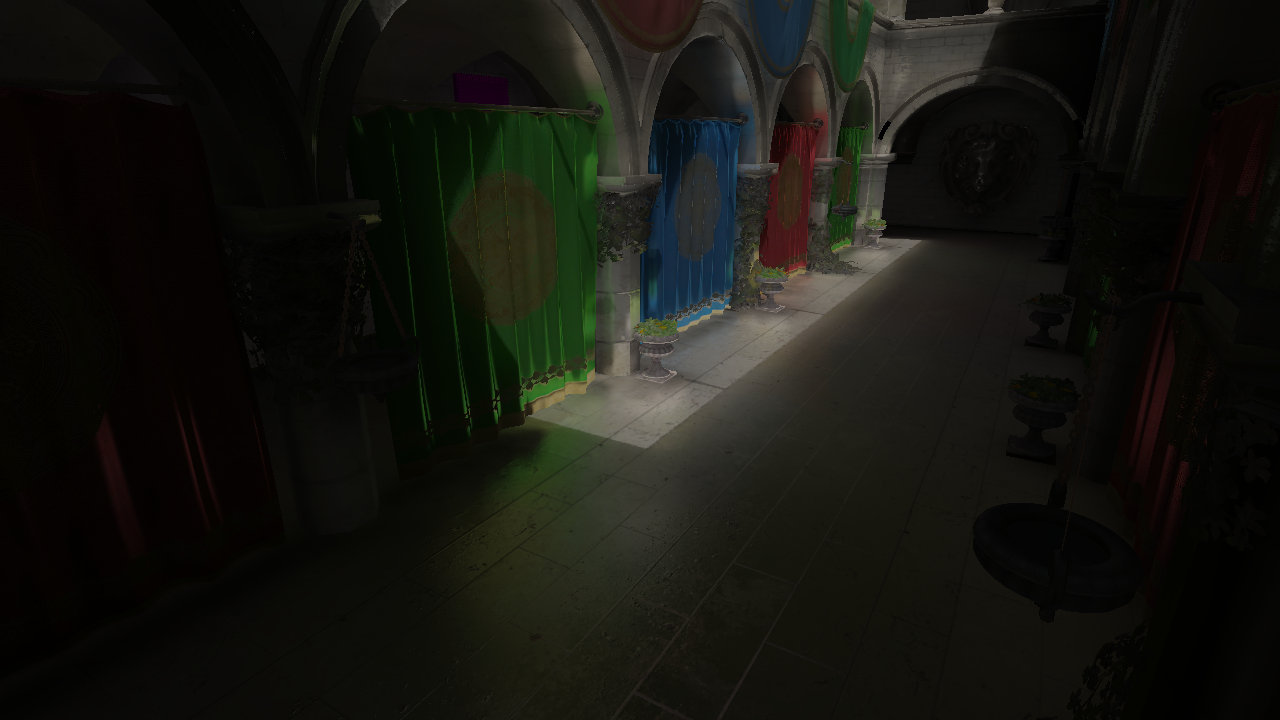
\includegraphics[width=\textwidth]{voxelwarp_off.png}
        \caption{Without voxel warping}
    \end{subfigure}
    ~
    \begin{subfigure}[t]{0.475\textwidth}
        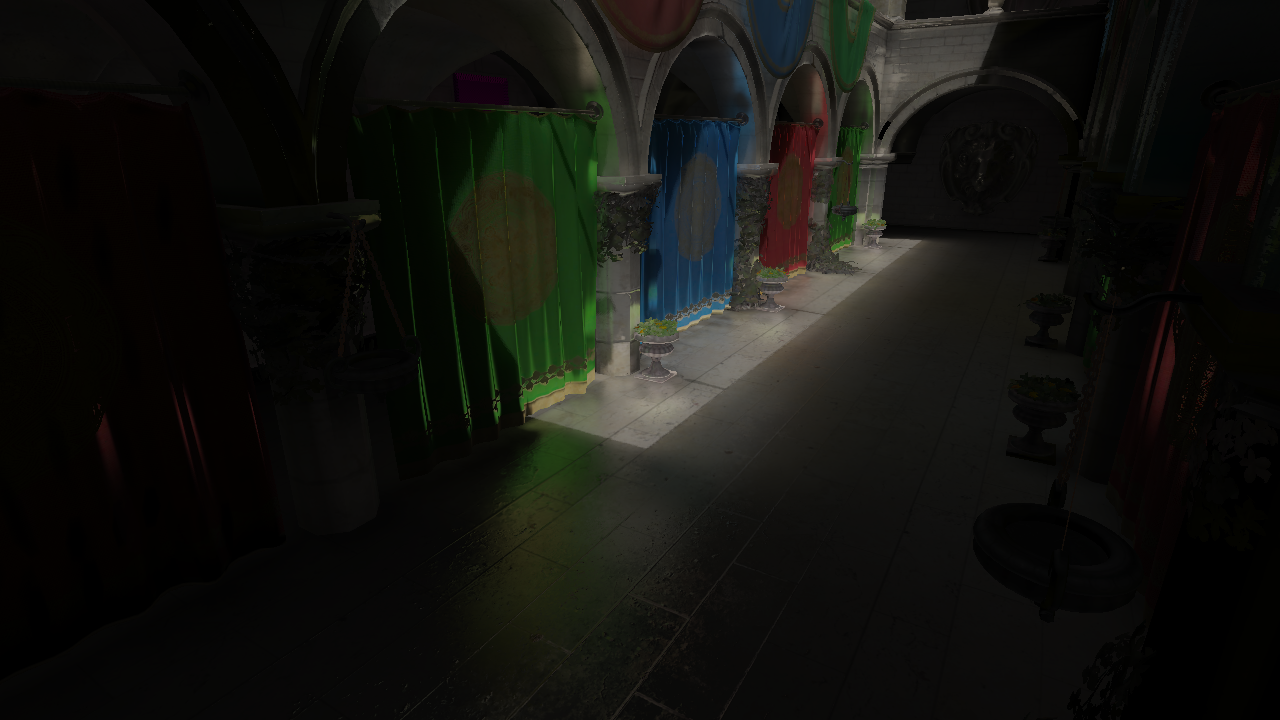
\includegraphics[width=\textwidth]{voxelwarp_on.png}
        \caption{With voxel warping}
    \end{subfigure}
    \caption{The voxel warping only has a small effect on lighting quality (the reflection of the green curtain is slightly more detailed).}
    \label{fig:results_voxelwarp}
\end{figure}

The second method of voxelization utilizes perspective projection to determine the voxel sizes. The motivation behind this is for voxel sizes to correspond to their respective sizes in screen space. The lighting quality for this approach is noticeably more detailed than with the warp function, as seen in Figure~\ref{fig:results_tesswarp}, however the temporal flickering issues are still apparent. With future work, we think this can be alleviated or eliminated.

\begin{figure}
    \centering
    \begin{subfigure}[t]{0.475\textwidth}
        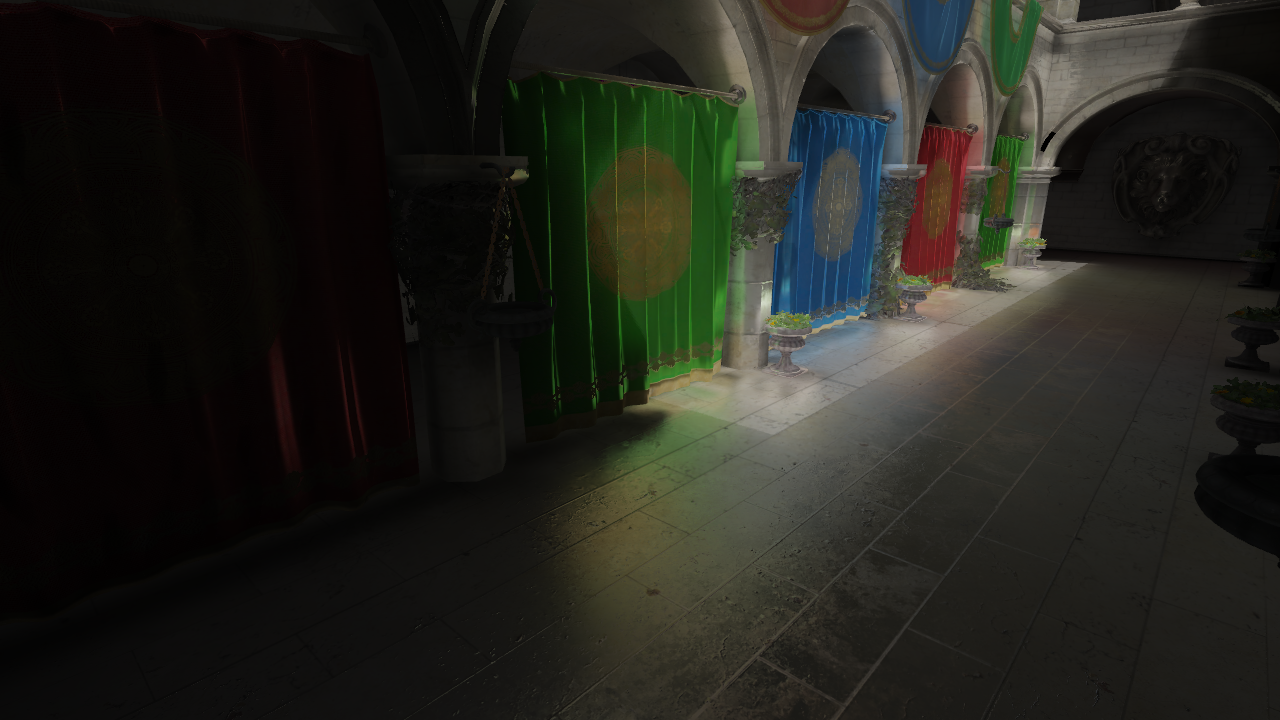
\includegraphics[width=\textwidth]{tesswarp_off.png}
        \caption{Without voxel warping}
    \end{subfigure}
    ~
    \begin{subfigure}[t]{0.475\textwidth}
        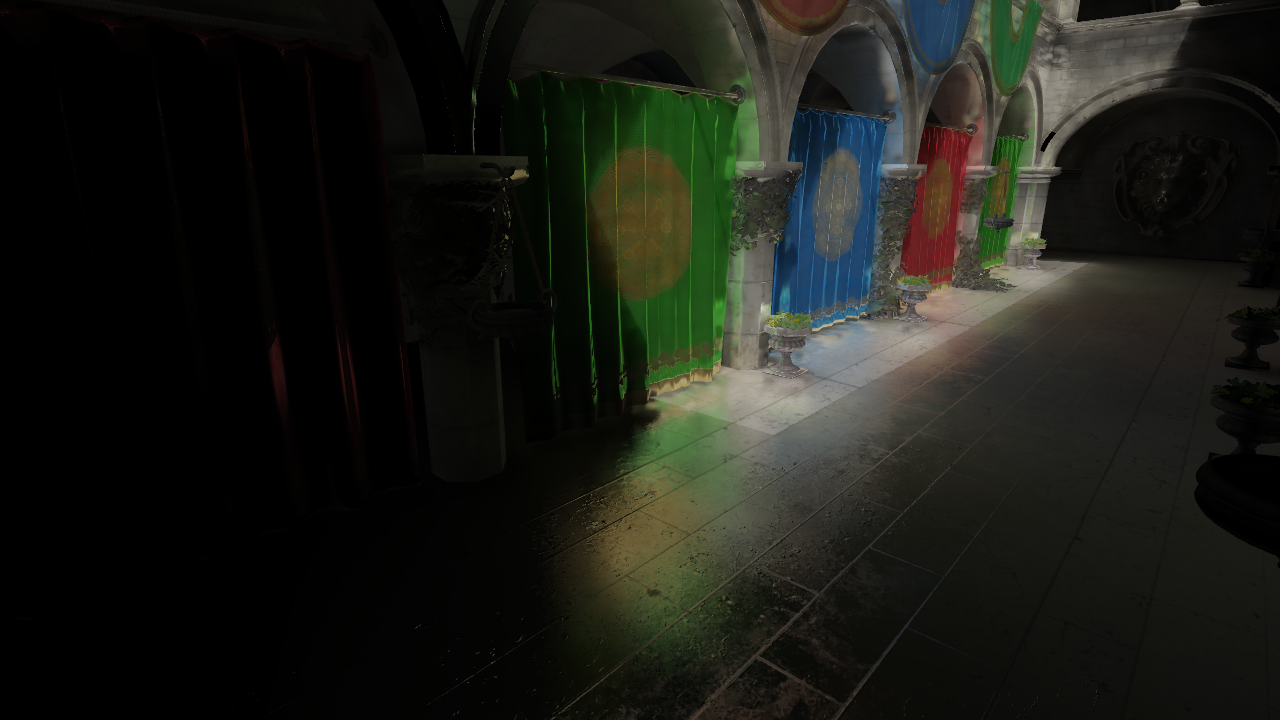
\includegraphics[width=\textwidth]{tesswarp_on.png}
        \caption{With voxel warping}
    \end{subfigure}
    \caption{The perspective voxel warping has a noticeable effect on lighting quality.}
    \label{fig:results_tesswarp}
\end{figure}

\chapter{Conclusions}

\begin{itemize}
    \item Developed GI solution
    \item Simple to implement and open source
    \item Competitive with existing solutions
    \item Voxel warping helps for larger scenes w/o significant performance/memory penalty
\end{itemize}

\section{Future Work}
Although voxel warping does help more efficiently use the space within a 3D texture, it can still suffer from wasted space when voxelizing a sparse scene (which leads to wasted GPU memory). An interesting way to solve this could be to utilize sparse textures (provided via the \verb#ARB_sparse_texture# extension for OpenGL). Sparse textures are analogous to classic virtual memory systems: not all parts of the texture are actually allocated in memory. Then, only the parts of the voxel texture that are used would require memory (of course the implementation allocates in fixed-size chunks, similar to pages in virtual memory).

Another potential area of improvement is storing radiance differently. For example, a spherical harmonics representation or ambient dice~\cite{iwanicki2017ambient} representation could be used. This would have impacts on both lighting quality, performance, and memory usage.

% TODO injecting multiple lights. can expand more on above stuff too

\nocite{*}
\bibliography{bibliography}

% Indents Appendix in Table of Contents
\makeatletter
\addtocontents{toc}{\let\protect\l@chapter\protect\l@section}
\makeatother

% Hack to make Appendices to appear in Table of Contents
% \addtocontents{toc}{%
%    \noindent APPENDICES
% }
% \begin{appendices}
% \input{appendix-outline}
% \end{appendices}

\end{document}
